\documentclass[letterpaper,11pt]{article}
\usepackage[margin=.65in,headheight=14pt,headsep=.16in,footskip=.3in]{geometry}
\usepackage[T1]{fontenc}
\usepackage{lmodern}
\pdfmapfile{+lm.map}
\usepackage{amsmath,amssymb,tikz,fancyhdr,enumitem,hyperref,textcomp}
\hypersetup{hidelinks,pdftitle={Week 15 Nearest site regions Facilitator guide},pdfauthor={Bellingham Math Circle}}
\pagestyle{fancy}\fancyhf{}
\fancyhead[L]{\small Bellingham Math Circle}\fancyhead[R]{\small Week 15 / Adult guide / Draft unpiloted}
\fancyfoot[L]{\small Nearest-site regions}\fancyfoot[R]{\small\thepage}
\renewcommand{\headrulewidth}{0pt}\renewcommand{\footrulewidth}{0pt}
\setlength{\parindent}{0pt}\setlength{\parskip}{5pt}
\setlist[itemize]{leftmargin=1.3em,itemsep=3pt,topsep=3pt}
\setlist[enumerate]{leftmargin=1.5em,itemsep=3pt,topsep=3pt}
\newcommand{\heading}[1]{\par\vspace{5pt}{\large\bfseries #1}\par}
\begin{document}{\Large\bfseries Nearest sites mathematical overview}\par
\textbf{Setting.} Take finitely many distinct sites in the Euclidean plane. A point belongs to every nearest site, so cells include shared boundaries. Sites are fixed within a map, and distance is to their centers. The printed frame is a window unless a problem explicitly restricts the target to it.

\textbf{Two sites and many sites.} For distinct sites $a,b$, points at equal distance form their perpendicular bisector; the closed half-plane on $a$'s side consists of points at least as close to $a$ as to $b$. The cell of $a$ is the intersection of these half-planes over every other site. It is convex and contains $a$, but can be unbounded. A pairwise equality is part of a shared cell boundary only where no third site is nearer. Three-way and higher ties are allowed.

\textbf{Changing and prescribing cells.} Adding a site adds a constraint to each old cell, so old cells can shrink or stay the same but cannot grow. To realize a convex polygon as the full cell of a site strictly inside it, reflect that site across each supporting edge line and place a competitor at each image. Intersecting the corresponding half-planes gives exactly the polygon. A nonconvex region cannot be one cell. Each distinct straight edge of a full polygonal cell requires a different competitor, giving a lower bound in minimum-site tasks.

\textbf{Across the bands.} K--1 compares lengths, records all tied letters and investigates simple placements. Grades 2--3 builds whole regions and sees how a third site changes a two-site boundary. Grades 4--5 explains half-plane intersections, insertion, convexity and inverse constructions. Coordinates and squared-distance algebra are adult checks, not prerequisites.

\textbf{Experiment and proof.} String comparisons and folds reveal patterns and suggest conjectures. Exact symmetry, perpendicular-bisector arguments and intersections justify an entire boundary or region. A few sampled points cannot prove a whole region is correct. Keep the theorem map with adults during the initial search; the preparation, longer explanations and all 24 problem solutions follow.
\newpage
{\LARGE\bfseries Nearest site regions}\par
{\large Facilitator guide for Week 15}\par
\textbf{Draft and unpiloted.} This adult guide accompanies the finalized three eight-page student packets, with Problems 1--8 in each. Week 15 is a library label, not a scheduled event. The guide is a separate, untested teaching step. Student pages are unchanged.

\heading{What the children are exploring}
A place belongs to every site that is nearest to it. Two sites give a straight dividing line; other sites can erase parts of that line. Whole regions come from satisfying all comparisons at once. Children can discover these ideas through string comparisons, folds and drawings; the coordinates in this guide are adult checks, not prerequisites.

\heading{Prerequisites and flexible entry points}
\begin{itemize}
\item \textbf{K--1:} compare two lengths and follow a spoken rule. Adult reads aloud and can scribe letters. No number reading, ruler arithmetic or coordinates needed.
\item \textbf{Grades 2--3:} compare several lengths, draw straight lines and keep all tied winners. Explain with a drawing or a spoken example; numerical measurement is optional.
\item \textbf{Grades 4--5:} reason about all points, overlapping allowed sides, possibility and a minimum. Algebra and formal proof notation are optional adult tools.
\end{itemize}
Grade labels are flexible. Offer a page based on readiness and interest. A child may spend the working time on two rich maps; finishing the packet is not the goal.

\heading{Practical preparation for ten children and three adults}
Print selected student pages single-sided, US Letter, at 100\% scale. Each working map is 5.8 inches across. Start with just one or two pages per child; hold the remaining pages in reserve. Make one adult copy of this guide and the relevant key pages for each table.

Prepare 10 pencils and erasers, 10 straightedges, 10 pieces of non-stretch string about 12 inches long, 40 sheets of translucent foldable paper, and 20 blank Letter sheets. Three colored pencils per child are optional; letters or hatching work equally well. These are preparation quantities, not checked inventory. Pre-cut string and try one fold before the meeting. Compare to the printed dot centers, not their circles or labels. Keep string on the table.

\heading{A flexible hour}
\begin{itemize}
\item \textbf{0--4 minutes:} freely try string comparisons and folds on spare paper.
\item \textbf{4--8:} launch together. Put two dots on a blank sheet; let a child choose a place and compare its straight lengths. Record A, B or AB. Say, ``We are finding every place that belongs to each dot. Tied nearest dots share the place.'' Demonstrate the recording, not the whole map.
\item \textbf{8--28:} work at three adult-led tables. Start with Problem 1; then K--1: 2 or 3; grades 2--3: 2 then 3; grades 4--5: 2 then 3. Offer a fold only if useful.
\item \textbf{28--31:} pause, stand and stretch. Two children act as fixed sites while another points to where a tie might be. Treat this as an estimate, not an exact measurement.
\item \textbf{31--52:} choose a branch: squares and insertion (K 5--6, middle 4--6, upper 4--5), or making a target (K 7--8, middle 7--8, upper 6--8). Save unfinished maps.
\item \textbf{52--60:} share a surprising tie or changed boundary. Ask for one drawing or physical reason; leave time to pack up.
\end{itemize}
\newpage
\begingroup\fontsize{10.5}{12.4}\selectfont
{\Large\bfseries Adult mathematical reference}\par
\heading{Shared conventions and fidelity limits}
All sites are distinct points and stay fixed within one map; placement problems add new sites without moving printed ones. Distance is straight-line distance in a flat plane, not grid travel. A cell is \emph{closed}: a point belongs to every nearest site. A two-way equality is not enough if a third site is nearer. The rectangular frame is only a window, except where a task explicitly compares a target inside it.

String and folding give evidence. Exact symmetry and the arguments below settle ties; do not turn printing or folding error into a new mathematical rule. Guide maps are reduced answer diagrams, not measurement masters. Use the original full-size student maps for children. Throughout the answer key, adult coordinates put the frame at $[-3,3]\times[-3,3]$, with $x$ right and $y$ up. A star marks a site added in one valid construction; inverse tasks can have other answers.

\heading{Why the methods work}
\textbf{Two sites.} Folding A onto B gives their perpendicular bisector. Reflection swaps A and B and fixes the crease, proving equality there. Each side is nearer its own site (see upper Problem 1). Only the crease ties.

\textbf{Several sites.} Keep the winning closed half-plane for one site against each competitor, then overlap those allowed sides. A surviving shared edge must also pass every other comparison. This explains why a third competitor can erase a pairwise bisector.

\textbf{Convexity.} A half-plane contains the entire segment between any two of its points. If both endpoints pass every comparison, so does their segment. Thus a cell cannot have a hole or an inward notch. This does not require children to know the word ``convex.''

\textbf{Insertion.} Adding a site adds a restriction for each old site. Old cells can shrink or stay the same; they cannot grow. Boundaries may disappear, but endpoints that remain nearest ties must be kept.

\textbf{Inverse construction.} To make an edge for A, reflect A across that edge and use its image as a competitor. The edge is then the bisector. Intersect all the chosen A-sides. This works for a convex polygon with A strictly inside it; it cannot make a nonconvex cell.

\textbf{Optional algebra.} For sites $a,b$ and test point $z$, squaring the nonnegative lengths and cancelling $z\cdot z$ gives
\[|z-a|^2\leq|z-b|^2\quad\Longleftrightarrow\quad 2(b-a)\cdot z\leq |b|^2-|a|^2.\]
This supplies the exact half-plane checks used for the answer diagrams.

\heading{Use hints sparingly and observe}
Let children make and test a proposal before offering the hint printed with each answer. Accept a fold, a drawing or a spoken argument. Ask ``Is some other dot closer?'' when an extra bisector remains; ``Does the region really stop there?'' when the frame is mistaken for a boundary. Record which pages were used, what children tried, and where adult rescue was needed. Classroom effectiveness remains unverified.

\heading{Sources and scope of adaptation}
\textbf{Mathematical reference:} David M. Mount, \emph{CMSC 754 Lecture 10: Voronoi Diagrams and Fortune's Algorithm}, Fall 2021, pp. 1--3. The definition, half-plane description, convexity and nearest-tie circle interpretation inform this lesson. The source uses open cells and assumes no four cocircular sites for its three-edge vertex claim. Here cells include their boundaries, and the square intentionally has a four-way meeting. The concrete arrangements, inverse examples, proofs and answer checks are independently worked for these packets.\par
{\small\url{https://www.cs.umd.edu/class/fall2021/cmsc754/Lects/lect10-vor.pdf}}\par
\textbf{Pedagogical consultation:} Natasha Rozhkovskaya, \emph{Math Circles for Elementary School Students}, ``Introduction: Berkeley 2009'' (local EPUB, section beginning with that heading). It describes individual adult attention, two additional instructors, and parents helping children and distributing handouts. The pacing, launch and hint choices here are new suggestions shaped by this project's concrete-first guidance, not a reported trial of this activity or a copied lesson from that book.
\endgroup

\newpage
{\Large\bfseries K--1 solutions}\par
\vspace{.08in}
{\large\bfseries Problem 1 Compare lengths}\par
\vspace{3pt}
\noindent\begin{minipage}[t]{.58\textwidth}\vspace{0pt}
\fontsize{10.8}{13.2}\selectfont
\textbf{Solution.} All crosses left of the vertical middle line get A; all right get B. The three crosses on the line get AB. The diagram labels all 16 answers (7 A, 6 B, 3 AB).

\textbf{Reasoning.} The two sites are mirror images in the middle line. Equal height does not determine the winner; distance to each center does.

\textbf{Hint to hold.} Hold one end of a string on a cross, pinch its length to A, then swing the same length toward B.

\textbf{Optional extension.} Invite a child to choose a new cross whose answer is AB.
\end{minipage}\hfill\begin{minipage}[t]{.40\textwidth}\vspace{0pt}\centering
\begin{tikzpicture}[x=.445in,y=.445in]
\path[use as bounding box] (-3.16,-3.2) rectangle (3.2,3.2);
\begin{scope}
\clip (-3,-3) rectangle (3,3);
\draw[line width=.7pt] (-3.00000000,-3.00000000)--(0.00000000,-3.00000000)--(0.00000000,3.00000000)--(-3.00000000,3.00000000)--cycle;
\draw[line width=.7pt] (0.00000000,-3.00000000)--(3.00000000,-3.00000000)--(3.00000000,3.00000000)--(0.00000000,3.00000000)--cycle;

\end{scope}
\draw[black!50,line width=.5pt] (-3,-3) rectangle (3,3);
\draw[line width=.6pt] (-2.555,2.3)--(-2.445,2.3) (-2.5,2.2449999999999997)--(-2.5,2.355);
\node[anchor=south west,fill=white,inner sep=.8pt,font=\sffamily\fontsize{7.6}{8.4}\selectfont] at (-2.4,2.3899999999999997) {A};
\draw[line width=.6pt] (-1.4549999999999998,1.2)--(-1.345,1.2) (-1.4,1.145)--(-1.4,1.255);
\node[anchor=south west,fill=white,inner sep=.8pt,font=\sffamily\fontsize{7.6}{8.4}\selectfont] at (-1.2999999999999998,1.29) {A};
\draw[line width=.6pt] (-0.6050000000000001,2.4)--(-0.49500000000000005,2.4) (-0.55,2.3449999999999998)--(-0.55,2.455);
\node[anchor=north west,fill=white,inner sep=.8pt,font=\sffamily\fontsize{7.6}{8.4}\selectfont] at (-0.45000000000000007,2.31) {A};
\draw[line width=.6pt] (-0.055,2.6)--(0.055,2.6) (0,2.545)--(0,2.6550000000000002);
\node[anchor=north west,fill=white,inner sep=.8pt,font=\sffamily\fontsize{7.6}{8.4}\selectfont] at (0.1,2.5100000000000002) {AB};
\draw[line width=.6pt] (0.6449999999999999,1.3)--(0.755,1.3) (0.7,1.245)--(0.7,1.355);
\node[anchor=south west,fill=white,inner sep=.8pt,font=\sffamily\fontsize{7.6}{8.4}\selectfont] at (0.7999999999999999,1.3900000000000001) {B};
\draw[line width=.6pt] (2.3449999999999998,2.3)--(2.455,2.3) (2.4,2.2449999999999997)--(2.4,2.355);
\node[anchor=south east,fill=white,inner sep=.8pt,font=\sffamily\fontsize{7.6}{8.4}\selectfont] at (2.3,2.3899999999999997) {B};
\draw[line width=.6pt] (-2.605,-1.2)--(-2.4949999999999997,-1.2) (-2.55,-1.255)--(-2.55,-1.145);
\node[anchor=south west,fill=white,inner sep=.8pt,font=\sffamily\fontsize{7.6}{8.4}\selectfont] at (-2.4499999999999997,-1.1099999999999999) {A};
\draw[line width=.6pt] (-1.355,-2.25)--(-1.245,-2.25) (-1.3,-2.305)--(-1.3,-2.195);
\node[anchor=south west,fill=white,inner sep=.8pt,font=\sffamily\fontsize{7.6}{8.4}\selectfont] at (-1.2,-2.16) {A};
\draw[line width=.6pt] (-0.555,-0.9)--(-0.445,-0.9) (-0.5,-0.9550000000000001)--(-0.5,-0.845);
\node[anchor=south west,fill=white,inner sep=.8pt,font=\sffamily\fontsize{7.6}{8.4}\selectfont] at (-0.4,-0.81) {A};
\draw[line width=.6pt] (-0.055,0)--(0.055,0) (0,-0.055)--(0,0.055);
\node[anchor=south west,fill=white,inner sep=.8pt,font=\sffamily\fontsize{7.6}{8.4}\selectfont] at (0.1,0.09) {AB};
\draw[line width=.6pt] (-0.055,-2.5)--(0.055,-2.5) (0,-2.555)--(0,-2.445);
\node[anchor=south west,fill=white,inner sep=.8pt,font=\sffamily\fontsize{7.6}{8.4}\selectfont] at (0.1,-2.41) {AB};
\draw[line width=.6pt] (0.5449999999999999,-2.05)--(0.655,-2.05) (0.6,-2.105)--(0.6,-1.9949999999999999);
\node[anchor=south west,fill=white,inner sep=.8pt,font=\sffamily\fontsize{7.6}{8.4}\selectfont] at (0.7,-1.9599999999999997) {B};
\draw[line width=.6pt] (1.445,-0.8)--(1.555,-0.8) (1.5,-0.8550000000000001)--(1.5,-0.745);
\node[anchor=south west,fill=white,inner sep=.8pt,font=\sffamily\fontsize{7.6}{8.4}\selectfont] at (1.6,-0.7100000000000001) {B};
\draw[line width=.6pt] (2.445,-2.3)--(2.555,-2.3) (2.5,-2.355)--(2.5,-2.2449999999999997);
\node[anchor=south east,fill=white,inner sep=.8pt,font=\sffamily\fontsize{7.6}{8.4}\selectfont] at (2.4,-2.21) {B};
\draw[line width=.6pt] (2.5949999999999998,0.75)--(2.705,0.75) (2.65,0.695)--(2.65,0.805);
\node[anchor=south east,fill=white,inner sep=.8pt,font=\sffamily\fontsize{7.6}{8.4}\selectfont] at (2.55,0.84) {B};
\draw[line width=.6pt] (-2.605,0.75)--(-2.4949999999999997,0.75) (-2.55,0.695)--(-2.55,0.805);
\node[anchor=south west,fill=white,inner sep=.8pt,font=\sffamily\fontsize{7.6}{8.4}\selectfont] at (-2.4499999999999997,0.84) {A};
\draw[fill=white,line width=.7pt] (-2.00000000,0.00000000) circle[radius=.065];
\fill (-2.00000000,0.00000000) circle[radius=.021];
\node[anchor=south west,fill=white,inner sep=.8pt,font=\bfseries\fontsize{9}{10}\selectfont] at (-1.9,0.1) {A};
\draw[fill=white,line width=.7pt] (2.00000000,0.00000000) circle[radius=.065];
\fill (2.00000000,0.00000000) circle[radius=.021];
\node[anchor=south west,fill=white,inner sep=.8pt,font=\bfseries\fontsize{9}{10}\selectfont] at (2.1,0.1) {B};
\end{tikzpicture}
\par\raggedright\fontsize{9}{11}\selectfont Small letters beside crosses give every nearest site.
\end{minipage}
\vfill
{\large\bfseries Problem 2 An oblique dividing line}\par
\vspace{3pt}
\noindent\begin{minipage}[t]{.58\textwidth}\vspace{0pt}
\fontsize{10.8}{13.2}\selectfont
\textbf{Solution.} The whole boundary is the sloping line through the center shown at right. A owns its lower-left side, B its upper-right side; both own the line.

\textbf{Reasoning.} Fold A exactly onto B. Every crease point stays in place while A and B swap, so its two lengths agree. The nearer side is the side containing that site. Adult check: $3x+2y=0$.

\textbf{Hint to hold.} If folding is awkward, trace the dots on translucent paper first.

\textbf{Optional extension.} Choose two far-apart places on the crease and check them with string.
\end{minipage}\hfill\begin{minipage}[t]{.40\textwidth}\vspace{0pt}\centering
\begin{tikzpicture}[x=.445in,y=.445in]
\path[use as bounding box] (-3.16,-3.2) rectangle (3.2,3.2);
\begin{scope}
\clip (-3,-3) rectangle (3,3);
\draw[line width=.7pt] (-3.00000000,-3.00000000)--(2.00000000,-3.00000000)--(-2.00000000,3.00000000)--(-3.00000000,3.00000000)--cycle;
\draw[line width=.7pt] (2.00000000,-3.00000000)--(3.00000000,-3.00000000)--(3.00000000,3.00000000)--(-2.00000000,3.00000000)--cycle;

\end{scope}
\draw[black!50,line width=.5pt] (-3,-3) rectangle (3,3);
\draw[fill=white,line width=.7pt] (-1.50000000,-1.00000000) circle[radius=.065];
\fill (-1.50000000,-1.00000000) circle[radius=.021];
\node[anchor=south west,fill=white,inner sep=.8pt,font=\bfseries\fontsize{9}{10}\selectfont] at (-1.4,-0.9) {A};
\draw[fill=white,line width=.7pt] (1.50000000,1.00000000) circle[radius=.065];
\fill (1.50000000,1.00000000) circle[radius=.021];
\node[anchor=south west,fill=white,inner sep=.8pt,font=\bfseries\fontsize{9}{10}\selectfont] at (1.6,1.1) {B};
\end{tikzpicture}
\par\raggedright\fontsize{9}{11}\selectfont The boundary reaches the top and bottom at $(-2,3)$ and $(2,-3)$.
\end{minipage}
\vspace{.15in}
\newpage
{\Large\bfseries K--1 solutions}\par
\vspace{.08in}
{\large\bfseries Problem 3 A middle strip}\par
\vspace{3pt}
\noindent\begin{minipage}[t]{.58\textwidth}\vspace{0pt}
\fontsize{10.8}{13.2}\selectfont
\textbf{Solution.} A owns $x\leq-1$; B owns $-1\leq x\leq1$; C owns $x\geq1$. The left line is shared by AB, the right by BC. There is no AC nearest tie.

\textbf{Reasoning.} The two adjacent midlines bound the middle strip. On the line halfway between A and C, B is closer than either outside site.

\textbf{Hint to hold.} After one pair agrees on a length, check that length against the third dot.

\textbf{Optional extension.} Ask whether a place very high above the middle dot still belongs to B.
\end{minipage}\hfill\begin{minipage}[t]{.40\textwidth}\vspace{0pt}\centering
\begin{tikzpicture}[x=.445in,y=.445in]
\path[use as bounding box] (-3.16,-3.2) rectangle (3.2,3.2);
\begin{scope}
\clip (-3,-3) rectangle (3,3);
\draw[line width=.7pt] (-3.00000000,-3.00000000)--(-1.00000000,-3.00000000)--(-1.00000000,3.00000000)--(-3.00000000,3.00000000)--cycle;
\draw[line width=.7pt] (-1.00000000,-3.00000000)--(1.00000000,-3.00000000)--(1.00000000,3.00000000)--(-1.00000000,3.00000000)--cycle;
\draw[line width=.7pt] (1.00000000,-3.00000000)--(3.00000000,-3.00000000)--(3.00000000,3.00000000)--(1.00000000,3.00000000)--cycle;

\end{scope}
\draw[black!50,line width=.5pt] (-3,-3) rectangle (3,3);
\draw[fill=white,line width=.7pt] (-2.00000000,0.00000000) circle[radius=.065];
\fill (-2.00000000,0.00000000) circle[radius=.021];
\node[anchor=south west,fill=white,inner sep=.8pt,font=\bfseries\fontsize{9}{10}\selectfont] at (-1.9,0.1) {A};
\draw[fill=white,line width=.7pt] (0.00000000,0.00000000) circle[radius=.065];
\fill (0.00000000,0.00000000) circle[radius=.021];
\node[anchor=south west,fill=white,inner sep=.8pt,font=\bfseries\fontsize{9}{10}\selectfont] at (0.1,0.1) {B};
\draw[fill=white,line width=.7pt] (2.00000000,0.00000000) circle[radius=.065];
\fill (2.00000000,0.00000000) circle[radius=.021];
\node[anchor=south west,fill=white,inner sep=.8pt,font=\bfseries\fontsize{9}{10}\selectfont] at (2.1,0.1) {C};
\end{tikzpicture}
\par\raggedright\fontsize{9}{11}\selectfont The strip continues beyond both ends of the printed frame.
\end{minipage}
\vfill
{\large\bfseries Problem 4 Three competitors}\par
\vspace{3pt}
\noindent\begin{minipage}[t]{.58\textwidth}\vspace{0pt}
\fontsize{10.8}{13.2}\selectfont
\textbf{Solution.} The top region belongs to C; the lower-left to A and lower-right to B. All 12 cross answers are marked. Counts: 3 A, 3 B, 1 C, 2 AB, 1 AC, 1 BC and 1 ABC.

\textbf{Reasoning.} The upper central cross belongs only to C even though its A and B lengths agree. The center belongs to ABC. The lower vertical ray is AB; the upper sloping rays are AC and BC.

\textbf{Hint to hold.} For a proposed tie, ask whether another dot is even nearer.

\textbf{Optional extension.} Make one new cross for each kind of answer that occurs.
\end{minipage}\hfill\begin{minipage}[t]{.40\textwidth}\vspace{0pt}\centering
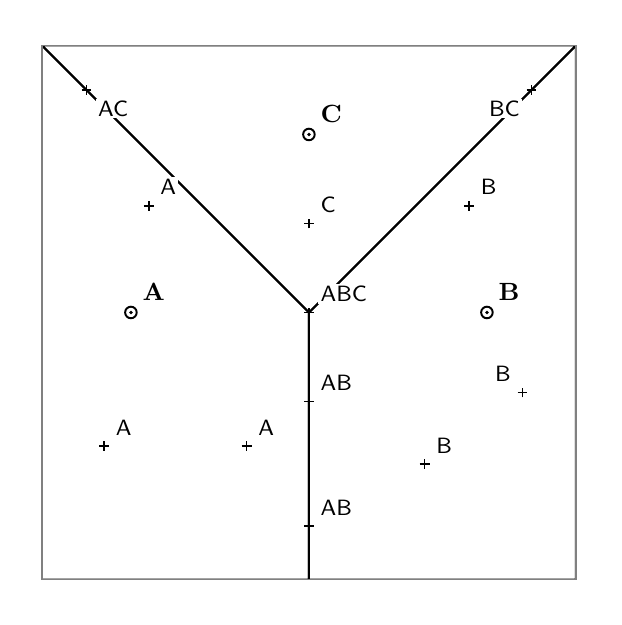
\begin{tikzpicture}[x=.445in,y=.445in]
\path[use as bounding box] (-3.16,-3.2) rectangle (3.2,3.2);
\begin{scope}
\clip (-3,-3) rectangle (3,3);
\draw[line width=.7pt] (-3.00000000,-3.00000000)--(0.00000000,-3.00000000)--(0.00000000,0.00000000)--(-3.00000000,3.00000000)--cycle;
\draw[line width=.7pt] (0.00000000,-3.00000000)--(3.00000000,-3.00000000)--(3.00000000,3.00000000)--(0.00000000,0.00000000)--cycle;
\draw[line width=.7pt] (3.00000000,3.00000000)--(-3.00000000,3.00000000)--(0.00000000,0.00000000)--cycle;

\end{scope}
\draw[black!50,line width=.5pt] (-3,-3) rectangle (3,3);
\draw[line width=.6pt] (-2.555,2.5)--(-2.445,2.5) (-2.5,2.445)--(-2.5,2.555);
\node[anchor=north west,fill=white,inner sep=.8pt,font=\sffamily\fontsize{7.6}{8.4}\selectfont] at (-2.4,2.41) {AC};
\draw[line width=.6pt] (-1.855,1.2)--(-1.745,1.2) (-1.8,1.145)--(-1.8,1.255);
\node[anchor=south west,fill=white,inner sep=.8pt,font=\sffamily\fontsize{7.6}{8.4}\selectfont] at (-1.7,1.29) {A};
\draw[line width=.6pt] (-0.055,1)--(0.055,1) (0,0.945)--(0,1.055);
\node[anchor=south west,fill=white,inner sep=.8pt,font=\sffamily\fontsize{7.6}{8.4}\selectfont] at (0.1,1.09) {C};
\draw[line width=.6pt] (1.745,1.2)--(1.855,1.2) (1.8,1.145)--(1.8,1.255);
\node[anchor=south west,fill=white,inner sep=.8pt,font=\sffamily\fontsize{7.6}{8.4}\selectfont] at (1.9000000000000001,1.29) {B};
\draw[line width=.6pt] (2.445,2.5)--(2.555,2.5) (2.5,2.445)--(2.5,2.555);
\node[anchor=north east,fill=white,inner sep=.8pt,font=\sffamily\fontsize{7.6}{8.4}\selectfont] at (2.4,2.41) {BC};
\draw[line width=.6pt] (-2.355,-1.5)--(-2.2449999999999997,-1.5) (-2.3,-1.555)--(-2.3,-1.445);
\node[anchor=south west,fill=white,inner sep=.8pt,font=\sffamily\fontsize{7.6}{8.4}\selectfont] at (-2.1999999999999997,-1.41) {A};
\draw[line width=.6pt] (-0.755,-1.5)--(-0.6449999999999999,-1.5) (-0.7,-1.555)--(-0.7,-1.445);
\node[anchor=south west,fill=white,inner sep=.8pt,font=\sffamily\fontsize{7.6}{8.4}\selectfont] at (-0.6,-1.41) {A};
\draw[line width=.6pt] (-0.055,-1)--(0.055,-1) (0,-1.055)--(0,-0.945);
\node[anchor=south west,fill=white,inner sep=.8pt,font=\sffamily\fontsize{7.6}{8.4}\selectfont] at (0.1,-0.91) {AB};
\draw[line width=.6pt] (1.245,-1.7)--(1.355,-1.7) (1.3,-1.755)--(1.3,-1.645);
\node[anchor=south west,fill=white,inner sep=.8pt,font=\sffamily\fontsize{7.6}{8.4}\selectfont] at (1.4000000000000001,-1.6099999999999999) {B};
\draw[line width=.6pt] (2.3449999999999998,-0.9)--(2.455,-0.9) (2.4,-0.9550000000000001)--(2.4,-0.845);
\node[anchor=south east,fill=white,inner sep=.8pt,font=\sffamily\fontsize{7.6}{8.4}\selectfont] at (2.3,-0.81) {B};
\draw[line width=.6pt] (-0.055,0)--(0.055,0) (0,-0.055)--(0,0.055);
\node[anchor=south west,fill=white,inner sep=.8pt,font=\sffamily\fontsize{7.6}{8.4}\selectfont] at (0.1,0.09) {ABC};
\draw[line width=.6pt] (-0.055,-2.4)--(0.055,-2.4) (0,-2.455)--(0,-2.3449999999999998);
\node[anchor=south west,fill=white,inner sep=.8pt,font=\sffamily\fontsize{7.6}{8.4}\selectfont] at (0.1,-2.31) {AB};
\draw[fill=white,line width=.7pt] (-2.00000000,0.00000000) circle[radius=.065];
\fill (-2.00000000,0.00000000) circle[radius=.021];
\node[anchor=south west,fill=white,inner sep=.8pt,font=\bfseries\fontsize{9}{10}\selectfont] at (-1.9,0.1) {A};
\draw[fill=white,line width=.7pt] (2.00000000,0.00000000) circle[radius=.065];
\fill (2.00000000,0.00000000) circle[radius=.021];
\node[anchor=south west,fill=white,inner sep=.8pt,font=\bfseries\fontsize{9}{10}\selectfont] at (2.1,0.1) {B};
\draw[fill=white,line width=.7pt] (0.00000000,2.00000000) circle[radius=.065];
\fill (0.00000000,2.00000000) circle[radius=.021];
\node[anchor=south west,fill=white,inner sep=.8pt,font=\bfseries\fontsize{9}{10}\selectfont] at (0.1,2.1) {C};
\end{tikzpicture}
\par\raggedright\fontsize{9}{11}\selectfont Closed cells: A: $x\leq0,\ y\leq-x$; B: $x\geq0,\ y\leq x$; C: $y\geq|x|$.
\end{minipage}
\vspace{.15in}
\newpage
{\Large\bfseries K--1 solutions}\par
\vspace{.08in}
{\large\bfseries Problem 5 Four regions can meet}\par
\vspace{3pt}
\noindent\begin{minipage}[t]{.58\textwidth}\vspace{0pt}
\fontsize{10.8}{13.2}\selectfont
\textbf{Solution.} The middle vertical and horizontal lines divide the map into four quarters: A upper-left, B upper-right, C lower-right, D lower-left. Their crossing belongs to all four.

\textbf{Reasoning.} Symmetry makes the center equally far from all four sites. On each half-axis, only the two adjacent quarters share a nearest tie; at the center all four do.

\textbf{Hint to hold.} Fold the left pair onto the right pair, then the top pair onto the bottom pair.

\textbf{Optional extension.} Have children find a place shared by exactly two dots.
\end{minipage}\hfill\begin{minipage}[t]{.40\textwidth}\vspace{0pt}\centering
\begin{tikzpicture}[x=.445in,y=.445in]
\path[use as bounding box] (-3.16,-3.2) rectangle (3.2,3.2);
\begin{scope}
\clip (-3,-3) rectangle (3,3);
\draw[line width=.7pt] (0.00000000,0.00000000)--(0.00000000,3.00000000)--(-3.00000000,3.00000000)--(-3.00000000,0.00000000)--cycle;
\draw[line width=.7pt] (3.00000000,0.00000000)--(3.00000000,3.00000000)--(0.00000000,3.00000000)--(0.00000000,0.00000000)--cycle;
\draw[line width=.7pt] (0.00000000,-3.00000000)--(3.00000000,-3.00000000)--(3.00000000,0.00000000)--(0.00000000,0.00000000)--cycle;
\draw[line width=.7pt] (-3.00000000,-3.00000000)--(0.00000000,-3.00000000)--(0.00000000,0.00000000)--(-3.00000000,0.00000000)--cycle;

\end{scope}
\draw[black!50,line width=.5pt] (-3,-3) rectangle (3,3);
\draw[fill=white,line width=.7pt] (-2.00000000,2.00000000) circle[radius=.065];
\fill (-2.00000000,2.00000000) circle[radius=.021];
\node[anchor=south west,fill=white,inner sep=.8pt,font=\bfseries\fontsize{9}{10}\selectfont] at (-1.9,2.1) {A};
\draw[fill=white,line width=.7pt] (2.00000000,2.00000000) circle[radius=.065];
\fill (2.00000000,2.00000000) circle[radius=.021];
\node[anchor=south west,fill=white,inner sep=.8pt,font=\bfseries\fontsize{9}{10}\selectfont] at (2.1,2.1) {B};
\draw[fill=white,line width=.7pt] (2.00000000,-2.00000000) circle[radius=.065];
\fill (2.00000000,-2.00000000) circle[radius=.021];
\node[anchor=south west,fill=white,inner sep=.8pt,font=\bfseries\fontsize{9}{10}\selectfont] at (2.1,-1.9) {C};
\draw[fill=white,line width=.7pt] (-2.00000000,-2.00000000) circle[radius=.065];
\fill (-2.00000000,-2.00000000) circle[radius=.021];
\node[anchor=south west,fill=white,inner sep=.8pt,font=\bfseries\fontsize{9}{10}\selectfont] at (-1.9,-1.9) {D};
\end{tikzpicture}
\par\raggedright\fontsize{9}{11}\selectfont Adjacent regions share rays; opposite regions meet only at the center.
\end{minipage}
\vfill
{\large\bfseries Problem 6 A new center takes a diamond}\par
\vspace{3pt}
\noindent\begin{minipage}[t]{.58\textwidth}\vspace{0pt}
\fontsize{10.8}{13.2}\selectfont
\textbf{Solution.} E gets the central diamond, including its edges. Each corner keeps the part of its old quarter outside the diamond. Its four vertices are three-way ties.

\textbf{Reasoning.} Compare E to each old site separately: four sloping midlines enclose E. Adult check: $|x|+|y|\leq2$. At $(0,2)$ the tie is ABE; at $(2,0)$ BCE; at $(0,-2)$ CDE; at $(-2,0)$ ADE.

\textbf{Hint to hold.} Find just the boundary between E and A before comparing E with the others.

\textbf{Optional extension.} Overlay Problems 5 and 6. Which old shared places no longer belong to either old neighbor?
\end{minipage}\hfill\begin{minipage}[t]{.40\textwidth}\vspace{0pt}\centering
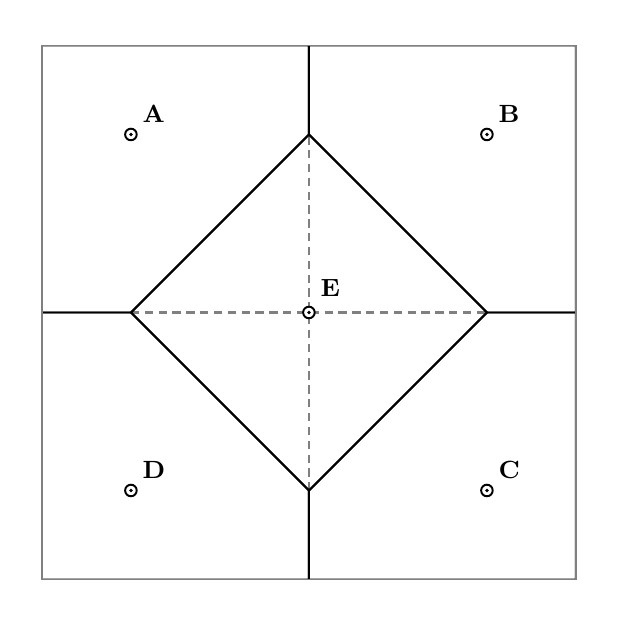
\begin{tikzpicture}[x=.445in,y=.445in]
\path[use as bounding box] (-3.16,-3.2) rectangle (3.2,3.2);
\begin{scope}
\clip (-3,-3) rectangle (3,3);
\draw[black!50,densely dashed,line width=.9pt] (-2,0)--(2,0) (0,-2)--(0,2);
\draw[line width=.7pt] (0.00000000,2.00000000)--(0.00000000,3.00000000)--(-3.00000000,3.00000000)--(-3.00000000,0.00000000)--(-2.00000000,0.00000000)--cycle;
\draw[line width=.7pt] (3.00000000,0.00000000)--(3.00000000,3.00000000)--(0.00000000,3.00000000)--(0.00000000,2.00000000)--(2.00000000,0.00000000)--cycle;
\draw[line width=.7pt] (0.00000000,-3.00000000)--(3.00000000,-3.00000000)--(3.00000000,0.00000000)--(2.00000000,0.00000000)--(0.00000000,-2.00000000)--cycle;
\draw[line width=.7pt] (-3.00000000,-3.00000000)--(0.00000000,-3.00000000)--(0.00000000,-2.00000000)--(-2.00000000,0.00000000)--(-3.00000000,0.00000000)--cycle;
\draw[line width=.7pt] (0.00000000,-2.00000000)--(2.00000000,0.00000000)--(0.00000000,2.00000000)--(-2.00000000,0.00000000)--cycle;

\end{scope}
\draw[black!50,line width=.5pt] (-3,-3) rectangle (3,3);
\draw[fill=white,line width=.7pt] (-2.00000000,2.00000000) circle[radius=.065];
\fill (-2.00000000,2.00000000) circle[radius=.021];
\node[anchor=south west,fill=white,inner sep=.8pt,font=\bfseries\fontsize{9}{10}\selectfont] at (-1.9,2.1) {A};
\draw[fill=white,line width=.7pt] (2.00000000,2.00000000) circle[radius=.065];
\fill (2.00000000,2.00000000) circle[radius=.021];
\node[anchor=south west,fill=white,inner sep=.8pt,font=\bfseries\fontsize{9}{10}\selectfont] at (2.1,2.1) {B};
\draw[fill=white,line width=.7pt] (2.00000000,-2.00000000) circle[radius=.065];
\fill (2.00000000,-2.00000000) circle[radius=.021];
\node[anchor=south west,fill=white,inner sep=.8pt,font=\bfseries\fontsize{9}{10}\selectfont] at (2.1,-1.9) {C};
\draw[fill=white,line width=.7pt] (-2.00000000,-2.00000000) circle[radius=.065];
\fill (-2.00000000,-2.00000000) circle[radius=.021];
\node[anchor=south west,fill=white,inner sep=.8pt,font=\bfseries\fontsize{9}{10}\selectfont] at (-1.9,-1.9) {D};
\draw[fill=white,line width=.7pt] (0.00000000,0.00000000) circle[radius=.065];
\fill (0.00000000,0.00000000) circle[radius=.021];
\node[anchor=south west,fill=white,inner sep=.8pt,font=\bfseries\fontsize{9}{10}\selectfont] at (0.1,0.15) {E};
\end{tikzpicture}
\par\raggedright\fontsize{9}{11}\selectfont Dashed segments were old boundaries; their four outer endpoints remain ties.
\end{minipage}
\vspace{.15in}
\newpage
{\Large\bfseries K--1 solutions}\par
\vspace{.08in}
{\large\bfseries Problem 7 Take places from both dots}\par
\vspace{3pt}
\noindent\begin{minipage}[t]{.58\textwidth}\vspace{0pt}
\fontsize{10.8}{13.2}\selectfont
\textbf{Solution.} One valid choice puts the new dot C at the midpoint of A and B. C then gets a sloping strip; A and B get the two outside sides. Other successful placements are welcome.

\textbf{Reasoning.} Near C on either side of the old A/B boundary, C is strictly closer. The new boundaries are the perpendicular bisectors of AC and BC. Adult check: C gets $|3x-2y|\leq39/10$.

\textbf{Hint to hold.} Where can you put a dot close to places from both old regions?

\textbf{Optional extension.} Let a partner propose a different placement and test a place taken from each old owner.
\end{minipage}\hfill\begin{minipage}[t]{.40\textwidth}\vspace{0pt}\centering
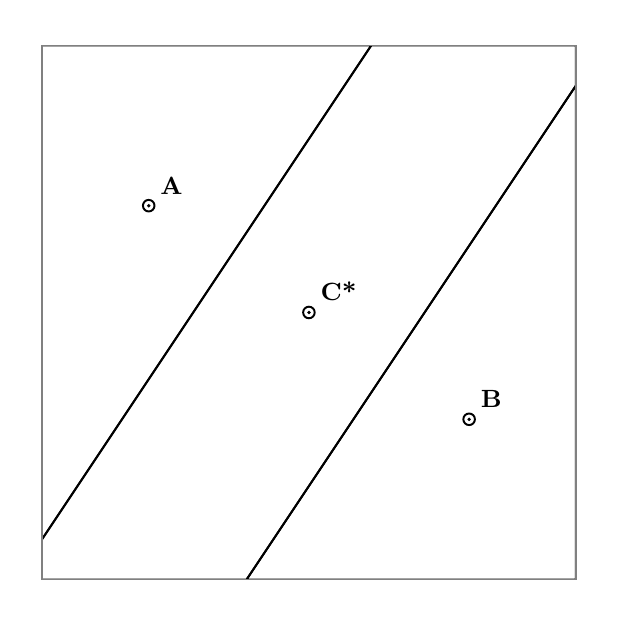
\begin{tikzpicture}[x=.445in,y=.445in]
\path[use as bounding box] (-3.16,-3.2) rectangle (3.2,3.2);
\begin{scope}
\clip (-3,-3) rectangle (3,3);
\draw[line width=.7pt] (0.70000000,3.00000000)--(-3.00000000,3.00000000)--(-3.00000000,-2.55000000)--cycle;
\draw[line width=.7pt] (-0.70000000,-3.00000000)--(3.00000000,-3.00000000)--(3.00000000,2.55000000)--cycle;
\draw[line width=.7pt] (-3.00000000,-3.00000000)--(-0.70000000,-3.00000000)--(3.00000000,2.55000000)--(3.00000000,3.00000000)--(0.70000000,3.00000000)--(-3.00000000,-2.55000000)--cycle;

\end{scope}
\draw[black!50,line width=.5pt] (-3,-3) rectangle (3,3);
\draw[fill=white,line width=.7pt] (-1.80000000,1.20000000) circle[radius=.065];
\fill (-1.80000000,1.20000000) circle[radius=.021];
\node[anchor=south west,fill=white,inner sep=.8pt,font=\bfseries\fontsize{9}{10}\selectfont] at (-1.7,1.3) {A};
\draw[fill=white,line width=.7pt] (1.80000000,-1.20000000) circle[radius=.065];
\fill (1.80000000,-1.20000000) circle[radius=.021];
\node[anchor=south west,fill=white,inner sep=.8pt,font=\bfseries\fontsize{9}{10}\selectfont] at (1.9000000000000001,-1.0999999999999999) {B};
\draw[fill=white,line width=.7pt] (0.00000000,0.00000000) circle[radius=.065];
\fill (0.00000000,0.00000000) circle[radius=.021];
\node[anchor=south west,fill=white,inner sep=.8pt,font=\bfseries\fontsize{9}{10}\selectfont] at (0.1,0.1) {C*};
\end{tikzpicture}
\par\raggedright\fontsize{9}{11}\selectfont C* is the added midpoint. Both strip edges are shared ties.
\end{minipage}
\vfill
{\large\bfseries Problem 8 Make the target strip}\par
\vspace{3pt}
\noindent\begin{minipage}[t]{.58\textwidth}\vspace{0pt}
\fontsize{10.8}{13.2}\selectfont
\textbf{Solution.} Place B at $(-2,0)$ and C at $(2,0)$, or exchange their names. A gets exactly the shaded strip in the frame, including both dashed target edges.

\textbf{Reasoning.} Each new site is the mirror image of A across one strip edge. Those edges become the two bisectors. Outside them, the respective new dot wins.

\textbf{Hint to hold.} Fold along one target edge. Where does the dot A land?

\textbf{Optional extension.} Choose a narrower strip around A and repeat on blank paper.
\end{minipage}\hfill\begin{minipage}[t]{.40\textwidth}\vspace{0pt}\centering
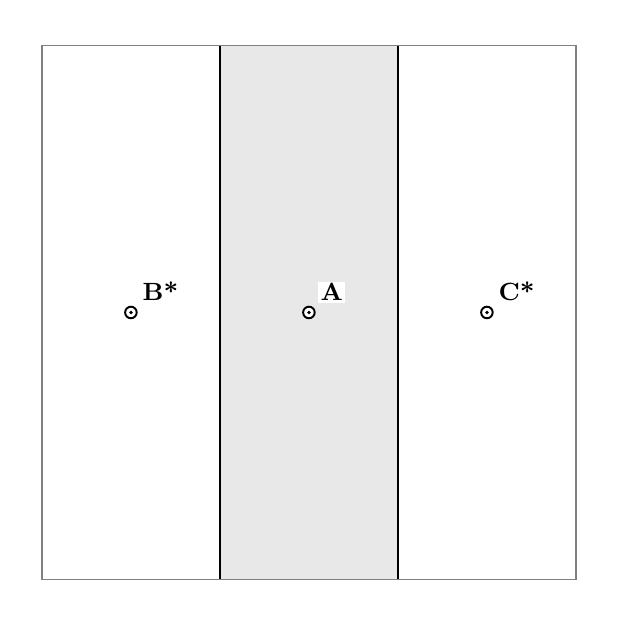
\begin{tikzpicture}[x=.445in,y=.445in]
\path[use as bounding box] (-3.16,-3.2) rectangle (3.2,3.2);
\fill[black!9] (-1.00000000,-3.00000000)--(1.00000000,-3.00000000)--(1.00000000,3.00000000)--(-1.00000000,3.00000000)--cycle;
\begin{scope}
\clip (-3,-3) rectangle (3,3);
\draw[line width=.7pt] (-1.00000000,-3.00000000)--(1.00000000,-3.00000000)--(1.00000000,3.00000000)--(-1.00000000,3.00000000)--cycle;

\end{scope}
\draw[black!50,line width=.5pt] (-3,-3) rectangle (3,3);
\draw[fill=white,line width=.7pt] (0.00000000,0.00000000) circle[radius=.065];
\fill (0.00000000,0.00000000) circle[radius=.021];
\node[anchor=south west,fill=white,inner sep=.8pt,font=\bfseries\fontsize{9}{10}\selectfont] at (0.1,0.1) {A};
\draw[fill=white,line width=.7pt] (-2.00000000,0.00000000) circle[radius=.065];
\fill (-2.00000000,0.00000000) circle[radius=.021];
\node[anchor=south west,fill=white,inner sep=.8pt,font=\bfseries\fontsize{9}{10}\selectfont] at (-1.9,0.1) {B*};
\draw[fill=white,line width=.7pt] (2.00000000,0.00000000) circle[radius=.065];
\fill (2.00000000,0.00000000) circle[radius=.021];
\node[anchor=south west,fill=white,inner sep=.8pt,font=\bfseries\fontsize{9}{10}\selectfont] at (2.1,0.1) {C*};
\end{tikzpicture}
\par\raggedright\fontsize{9}{11}\selectfont A owns $-1\leq x\leq1$. Its whole region is an infinite strip.
\end{minipage}
\vspace{.15in}
\newpage
{\Large\bfseries Grades 2--3 solutions}\par
\vspace{.08in}
{\large\bfseries Problem 1 From samples to a whole boundary}\par
\vspace{3pt}
\noindent\begin{minipage}[t]{.58\textwidth}\vspace{0pt}
\fontsize{10.8}{13.2}\selectfont
\textbf{Solution.} A wins at the 4 crosses with $x+y<0$; B at the 6 with $x+y>0$; the 4 with $x+y=0$ get AB. All 14 answers are shown. The full boundary is the descending diagonal.

\textbf{Reasoning.} The sites reflect across $x+y=0$. Testing crosses suggests the line; a fold or reflection explains the entire line and its two sides.

\textbf{Hint to hold.} Find two tied places far apart, then ask what might connect them.

\textbf{Optional extension.} Choose a point not printed and predict its answer before measuring.
\end{minipage}\hfill\begin{minipage}[t]{.40\textwidth}\vspace{0pt}\centering
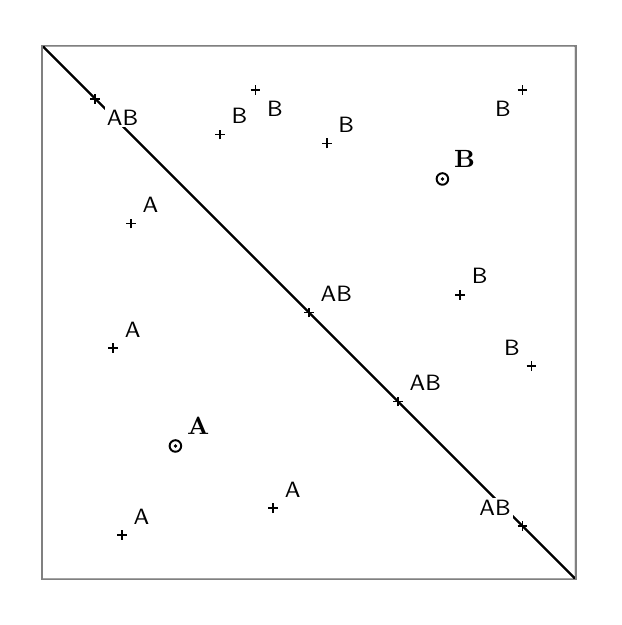
\begin{tikzpicture}[x=.445in,y=.445in]
\path[use as bounding box] (-3.16,-3.2) rectangle (3.2,3.2);
\begin{scope}
\clip (-3,-3) rectangle (3,3);
\draw[line width=.7pt] (-3.00000000,-3.00000000)--(3.00000000,-3.00000000)--(-3.00000000,3.00000000)--cycle;
\draw[line width=.7pt] (3.00000000,-3.00000000)--(3.00000000,3.00000000)--(-3.00000000,3.00000000)--cycle;

\end{scope}
\draw[black!50,line width=.5pt] (-3,-3) rectangle (3,3);
\draw[line width=.6pt] (-2.455,2.4)--(-2.3449999999999998,2.4) (-2.4,2.3449999999999998)--(-2.4,2.455);
\node[anchor=north west,fill=white,inner sep=.8pt,font=\sffamily\fontsize{7.6}{8.4}\selectfont] at (-2.3,2.31) {AB};
\draw[line width=.6pt] (-2.055,1)--(-1.945,1) (-2,0.945)--(-2,1.055);
\node[anchor=south west,fill=white,inner sep=.8pt,font=\sffamily\fontsize{7.6}{8.4}\selectfont] at (-1.9,1.09) {A};
\draw[line width=.6pt] (-1.055,2)--(-0.945,2) (-1,1.945)--(-1,2.055);
\node[anchor=south west,fill=white,inner sep=.8pt,font=\sffamily\fontsize{7.6}{8.4}\selectfont] at (-0.9,2.09) {B};
\draw[line width=.6pt] (-0.055,0)--(0.055,0) (0,-0.055)--(0,0.055);
\node[anchor=south west,fill=white,inner sep=.8pt,font=\sffamily\fontsize{7.6}{8.4}\selectfont] at (0.1,0.09) {AB};
\draw[line width=.6pt] (0.945,-1)--(1.055,-1) (1,-1.055)--(1,-0.945);
\node[anchor=south west,fill=white,inner sep=.8pt,font=\sffamily\fontsize{7.6}{8.4}\selectfont] at (1.1,-0.91) {AB};
\draw[line width=.6pt] (2.3449999999999998,-2.4)--(2.455,-2.4) (2.4,-2.455)--(2.4,-2.3449999999999998);
\node[anchor=south east,fill=white,inner sep=.8pt,font=\sffamily\fontsize{7.6}{8.4}\selectfont] at (2.3,-2.31) {AB};
\draw[line width=.6pt] (-2.2550000000000003,-0.4)--(-2.145,-0.4) (-2.2,-0.455)--(-2.2,-0.34500000000000003);
\node[anchor=south west,fill=white,inner sep=.8pt,font=\sffamily\fontsize{7.6}{8.4}\selectfont] at (-2.1,-0.31000000000000005) {A};
\draw[line width=.6pt] (-0.455,-2.2)--(-0.34500000000000003,-2.2) (-0.4,-2.2550000000000003)--(-0.4,-2.145);
\node[anchor=south west,fill=white,inner sep=.8pt,font=\sffamily\fontsize{7.6}{8.4}\selectfont] at (-0.30000000000000004,-2.1100000000000003) {A};
\draw[line width=.6pt] (-2.1550000000000002,-2.5)--(-2.045,-2.5) (-2.1,-2.555)--(-2.1,-2.445);
\node[anchor=south west,fill=white,inner sep=.8pt,font=\sffamily\fontsize{7.6}{8.4}\selectfont] at (-2.0,-2.41) {A};
\draw[line width=.6pt] (0.14500000000000002,1.9)--(0.255,1.9) (0.2,1.845)--(0.2,1.9549999999999998);
\node[anchor=south west,fill=white,inner sep=.8pt,font=\sffamily\fontsize{7.6}{8.4}\selectfont] at (0.30000000000000004,1.99) {B};
\draw[line width=.6pt] (1.645,0.2)--(1.755,0.2) (1.7,0.14500000000000002)--(1.7,0.255);
\node[anchor=south west,fill=white,inner sep=.8pt,font=\sffamily\fontsize{7.6}{8.4}\selectfont] at (1.8,0.29000000000000004) {B};
\draw[line width=.6pt] (2.3449999999999998,2.5)--(2.455,2.5) (2.4,2.445)--(2.4,2.555);
\node[anchor=north east,fill=white,inner sep=.8pt,font=\sffamily\fontsize{7.6}{8.4}\selectfont] at (2.3,2.41) {B};
\draw[line width=.6pt] (2.445,-0.6)--(2.555,-0.6) (2.5,-0.655)--(2.5,-0.5449999999999999);
\node[anchor=south east,fill=white,inner sep=.8pt,font=\sffamily\fontsize{7.6}{8.4}\selectfont] at (2.4,-0.51) {B};
\draw[line width=.6pt] (-0.655,2.5)--(-0.5449999999999999,2.5) (-0.6,2.445)--(-0.6,2.555);
\node[anchor=north west,fill=white,inner sep=.8pt,font=\sffamily\fontsize{7.6}{8.4}\selectfont] at (-0.5,2.41) {B};
\draw[fill=white,line width=.7pt] (-1.50000000,-1.50000000) circle[radius=.065];
\fill (-1.50000000,-1.50000000) circle[radius=.021];
\node[anchor=south west,fill=white,inner sep=.8pt,font=\bfseries\fontsize{9}{10}\selectfont] at (-1.4,-1.4) {A};
\draw[fill=white,line width=.7pt] (1.50000000,1.50000000) circle[radius=.065];
\fill (1.50000000,1.50000000) circle[radius=.021];
\node[anchor=south west,fill=white,inner sep=.8pt,font=\bfseries\fontsize{9}{10}\selectfont] at (1.6,1.6) {B};
\end{tikzpicture}
\par\raggedright\fontsize{9}{11}\selectfont AB crosses are $(-2.4,2.4)$, $(0,0)$, $(1,-1)$ and $(2.4,-2.4)$.
\end{minipage}
\vfill
{\large\bfseries Problem 2 An equality may lose}\par
\vspace{3pt}
\noindent\begin{minipage}[t]{.58\textwidth}\vspace{0pt}
\fontsize{10.8}{13.2}\selectfont
\textbf{Solution.} Three rays, rather than three complete lines, form the nearest-site boundaries. The center belongs to ABC.

\textbf{Reasoning.} A and B are equally far from every place on the vertical middle line. Below the center they are nearest; above it C is nearer. Keep only ties for nearest dots, including the three-way tie at the center.

\textbf{Hint to hold.} Check all three lengths before keeping any pairwise tie.

\textbf{Optional extension.} Find a point on the erased part of the A/B bisector.
\end{minipage}\hfill\begin{minipage}[t]{.40\textwidth}\vspace{0pt}\centering
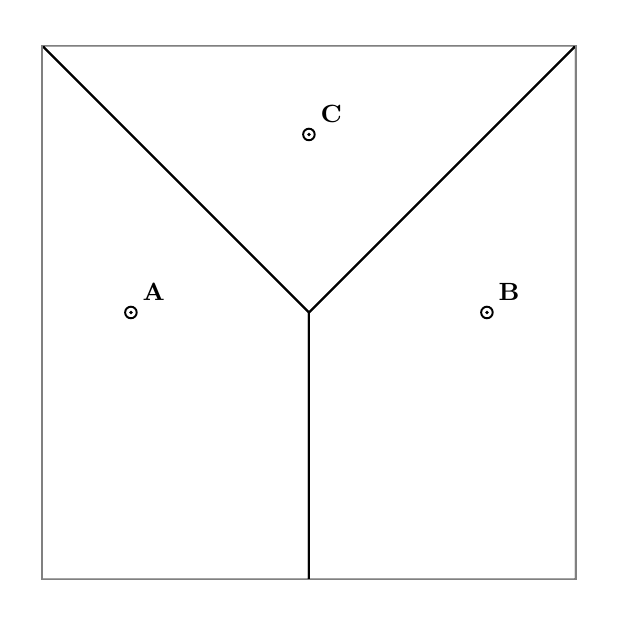
\begin{tikzpicture}[x=.445in,y=.445in]
\path[use as bounding box] (-3.16,-3.2) rectangle (3.2,3.2);
\begin{scope}
\clip (-3,-3) rectangle (3,3);
\draw[line width=.7pt] (-3.00000000,-3.00000000)--(0.00000000,-3.00000000)--(0.00000000,0.00000000)--(-3.00000000,3.00000000)--cycle;
\draw[line width=.7pt] (0.00000000,-3.00000000)--(3.00000000,-3.00000000)--(3.00000000,3.00000000)--(0.00000000,0.00000000)--cycle;
\draw[line width=.7pt] (3.00000000,3.00000000)--(-3.00000000,3.00000000)--(0.00000000,0.00000000)--cycle;

\end{scope}
\draw[black!50,line width=.5pt] (-3,-3) rectangle (3,3);
\draw[fill=white,line width=.7pt] (-2.00000000,0.00000000) circle[radius=.065];
\fill (-2.00000000,0.00000000) circle[radius=.021];
\node[anchor=south west,fill=white,inner sep=.8pt,font=\bfseries\fontsize{9}{10}\selectfont] at (-1.9,0.1) {A};
\draw[fill=white,line width=.7pt] (2.00000000,0.00000000) circle[radius=.065];
\fill (2.00000000,0.00000000) circle[radius=.021];
\node[anchor=south west,fill=white,inner sep=.8pt,font=\bfseries\fontsize{9}{10}\selectfont] at (2.1,0.1) {B};
\draw[fill=white,line width=.7pt] (0.00000000,2.00000000) circle[radius=.065];
\fill (0.00000000,2.00000000) circle[radius=.021];
\node[anchor=south west,fill=white,inner sep=.8pt,font=\bfseries\fontsize{9}{10}\selectfont] at (0.1,2.1) {C};
\end{tikzpicture}
\par\raggedright\fontsize{9}{11}\selectfont AB: $x=0,y\leq0$; AC: $y=-x,x\leq0$; BC: $y=x,x\geq0$.
\end{minipage}
\vspace{.15in}
\newpage
{\Large\bfseries Grades 2--3 solutions}\par
\vspace{.08in}
{\large\bfseries Problem 3 Unequal gaps on a line}\par
\vspace{3pt}
\noindent\begin{minipage}[t]{.58\textwidth}\vspace{0pt}
\fontsize{10.8}{13.2}\selectfont
\textbf{Solution.} A: $x\leq-5/4$; B: $-5/4\leq x\leq3/4$; C: $x\geq3/4$. The boundary lines are AB and BC, respectively. No place belongs to all three.

\textbf{Reasoning.} An AB tie would need $x=-5/4$, whereas a BC tie needs $x=3/4$. No point can have both horizontal coordinates. Equivalently, the two midlines are parallel and different.

\textbf{Hint to hold.} Compare the midpoints of the two neighboring gaps.

\textbf{Optional extension.} Move B along the line on a fresh map. Does a three-way tie ever appear while the sites stay distinct?
\end{minipage}\hfill\begin{minipage}[t]{.40\textwidth}\vspace{0pt}\centering
\begin{tikzpicture}[x=.445in,y=.445in]
\path[use as bounding box] (-3.16,-3.2) rectangle (3.2,3.2);
\begin{scope}
\clip (-3,-3) rectangle (3,3);
\draw[line width=.7pt] (-3.00000000,-3.00000000)--(-1.25000000,-3.00000000)--(-1.25000000,3.00000000)--(-3.00000000,3.00000000)--cycle;
\draw[line width=.7pt] (-1.25000000,-3.00000000)--(0.75000000,-3.00000000)--(0.75000000,3.00000000)--(-1.25000000,3.00000000)--cycle;
\draw[line width=.7pt] (0.75000000,-3.00000000)--(3.00000000,-3.00000000)--(3.00000000,3.00000000)--(0.75000000,3.00000000)--cycle;

\end{scope}
\draw[black!50,line width=.5pt] (-3,-3) rectangle (3,3);
\draw[fill=white,line width=.7pt] (-2.00000000,0.00000000) circle[radius=.065];
\fill (-2.00000000,0.00000000) circle[radius=.021];
\node[anchor=south west,fill=white,inner sep=.8pt,font=\bfseries\fontsize{9}{10}\selectfont] at (-1.9,0.1) {A};
\draw[fill=white,line width=.7pt] (-0.50000000,0.00000000) circle[radius=.065];
\fill (-0.50000000,0.00000000) circle[radius=.021];
\node[anchor=south west,fill=white,inner sep=.8pt,font=\bfseries\fontsize{9}{10}\selectfont] at (-0.4,0.1) {B};
\draw[fill=white,line width=.7pt] (2.00000000,0.00000000) circle[radius=.065];
\fill (2.00000000,0.00000000) circle[radius=.021];
\node[anchor=south west,fill=white,inner sep=.8pt,font=\bfseries\fontsize{9}{10}\selectfont] at (2.1,0.1) {C};
\end{tikzpicture}
\par\raggedright\fontsize{9}{11}\selectfont On the AC equality line $x=0$, the middle site B is closer.
\end{minipage}
\vfill
{\large\bfseries Problem 4 All shared places in the square}\par
\vspace{3pt}
\noindent\begin{minipage}[t]{.58\textwidth}\vspace{0pt}
\fontsize{10.8}{13.2}\selectfont
\textbf{Solution.} The cells are the four closed quarters shown. Every point of either central axis is shared: AB above, BC right, CD below, AD left. The center belongs to ABCD.

\textbf{Reasoning.} Horizontal and vertical symmetry supplies the boundaries. AC and BD share the center only, so shared points need not form a positive-length edge.

\textbf{Hint to hold.} At a proposed shared place, ask which of the four distances are shortest.

\textbf{Optional extension.} Compare with Problem 5: what changes when one corner moves?
\end{minipage}\hfill\begin{minipage}[t]{.40\textwidth}\vspace{0pt}\centering
\begin{tikzpicture}[x=.445in,y=.445in]
\path[use as bounding box] (-3.16,-3.2) rectangle (3.2,3.2);
\begin{scope}
\clip (-3,-3) rectangle (3,3);
\draw[line width=.7pt] (0.00000000,0.00000000)--(0.00000000,3.00000000)--(-3.00000000,3.00000000)--(-3.00000000,0.00000000)--cycle;
\draw[line width=.7pt] (3.00000000,0.00000000)--(3.00000000,3.00000000)--(0.00000000,3.00000000)--(0.00000000,0.00000000)--cycle;
\draw[line width=.7pt] (0.00000000,-3.00000000)--(3.00000000,-3.00000000)--(3.00000000,0.00000000)--(0.00000000,0.00000000)--cycle;
\draw[line width=.7pt] (-3.00000000,-3.00000000)--(0.00000000,-3.00000000)--(0.00000000,0.00000000)--(-3.00000000,0.00000000)--cycle;

\end{scope}
\draw[black!50,line width=.5pt] (-3,-3) rectangle (3,3);
\draw[fill=white,line width=.7pt] (-2.00000000,2.00000000) circle[radius=.065];
\fill (-2.00000000,2.00000000) circle[radius=.021];
\node[anchor=south west,fill=white,inner sep=.8pt,font=\bfseries\fontsize{9}{10}\selectfont] at (-1.9,2.1) {A};
\draw[fill=white,line width=.7pt] (2.00000000,2.00000000) circle[radius=.065];
\fill (2.00000000,2.00000000) circle[radius=.021];
\node[anchor=south west,fill=white,inner sep=.8pt,font=\bfseries\fontsize{9}{10}\selectfont] at (2.1,2.1) {B};
\draw[fill=white,line width=.7pt] (2.00000000,-2.00000000) circle[radius=.065];
\fill (2.00000000,-2.00000000) circle[radius=.021];
\node[anchor=south west,fill=white,inner sep=.8pt,font=\bfseries\fontsize{9}{10}\selectfont] at (2.1,-1.9) {C};
\draw[fill=white,line width=.7pt] (-2.00000000,-2.00000000) circle[radius=.065];
\fill (-2.00000000,-2.00000000) circle[radius=.021];
\node[anchor=south west,fill=white,inner sep=.8pt,font=\bfseries\fontsize{9}{10}\selectfont] at (-1.9,-1.9) {D};
\end{tikzpicture}
\par\raggedright\fontsize{9}{11}\selectfont This is also the counterexample to a blanket claim that only three cells can meet.
\end{minipage}
\vspace{.15in}
\newpage
{\Large\bfseries Grades 2--3 solutions}\par
\vspace{.08in}
{\large\bfseries Problem 5 A perturbed square}\par
\vspace{3pt}
\noindent\begin{minipage}[t]{.58\textwidth}\vspace{0pt}
\fontsize{10.8}{13.2}\selectfont
\textbf{Solution.} The sharing pairs are AB, AD, BC, BD and CD. AC has no shared point. The short BD edge joins $U=(0,-1/2)$ and $V=(3/8,0)$. U belongs to ABD; V to BCD.

\textbf{Reasoning.} The surviving outer rays are AB: $x=0,y\leq-1/2$; AD: $y=-1/2,x\leq0$; BC: $y=0,x\geq3/8$; CD: $4x+y=3/2,x\leq3/8$. BD is $y=4x/3-1/2$ between U and V.

\textbf{Hint to hold.} Inspect a small neighborhood near the middle, rather than extending every crease forever.

\textbf{Optional extension.} Compare the two three-way vertices with the single four-way vertex in Problem 4.
\end{minipage}\hfill\begin{minipage}[t]{.40\textwidth}\vspace{0pt}\centering
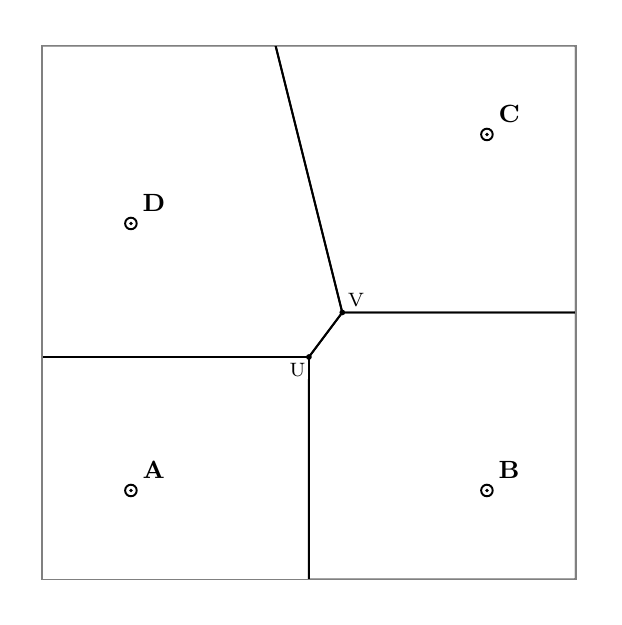
\begin{tikzpicture}[x=.445in,y=.445in]
\path[use as bounding box] (-3.16,-3.2) rectangle (3.2,3.2);
\begin{scope}
\clip (-3,-3) rectangle (3,3);
\draw[line width=.7pt] (-3.00000000,-3.00000000)--(0.00000000,-3.00000000)--(0.00000000,-0.50000000)--(-3.00000000,-0.50000000)--cycle;
\draw[line width=.7pt] (0.00000000,-3.00000000)--(3.00000000,-3.00000000)--(3.00000000,0.00000000)--(0.37500000,0.00000000)--(0.00000000,-0.50000000)--cycle;
\draw[line width=.7pt] (3.00000000,0.00000000)--(3.00000000,3.00000000)--(-0.37500000,3.00000000)--(0.37500000,0.00000000)--cycle;
\draw[line width=.7pt] (-0.37500000,3.00000000)--(-3.00000000,3.00000000)--(-3.00000000,-0.50000000)--(0.00000000,-0.50000000)--(0.37500000,0.00000000)--cycle;
\fill (0,-.5) circle[radius=.032] (.375,0) circle[radius=.032];\node[anchor=north east,font=\scriptsize,fill=white,inner sep=1pt] at (0,-.53) {U};\node[anchor=south west,font=\scriptsize,fill=white,inner sep=1pt] at (.4,.03) {V};
\end{scope}
\draw[black!50,line width=.5pt] (-3,-3) rectangle (3,3);
\draw[fill=white,line width=.7pt] (-2.00000000,-2.00000000) circle[radius=.065];
\fill (-2.00000000,-2.00000000) circle[radius=.021];
\node[anchor=south west,fill=white,inner sep=.8pt,font=\bfseries\fontsize{9}{10}\selectfont] at (-1.9,-1.9) {A};
\draw[fill=white,line width=.7pt] (2.00000000,-2.00000000) circle[radius=.065];
\fill (2.00000000,-2.00000000) circle[radius=.021];
\node[anchor=south west,fill=white,inner sep=.8pt,font=\bfseries\fontsize{9}{10}\selectfont] at (2.1,-1.9) {B};
\draw[fill=white,line width=.7pt] (2.00000000,2.00000000) circle[radius=.065];
\fill (2.00000000,2.00000000) circle[radius=.021];
\node[anchor=south west,fill=white,inner sep=.8pt,font=\bfseries\fontsize{9}{10}\selectfont] at (2.1,2.1) {C};
\draw[fill=white,line width=.7pt] (-2.00000000,1.00000000) circle[radius=.065];
\fill (-2.00000000,1.00000000) circle[radius=.021];
\node[anchor=south west,fill=white,inner sep=.8pt,font=\bfseries\fontsize{9}{10}\selectfont] at (-1.9,1.1) {D};
\end{tikzpicture}
\par\raggedright\fontsize{9}{11}\selectfont The BD segment has length $5/8$ map unit; it is not a four-way tie.
\end{minipage}
\vfill
{\large\bfseries Problem 6 Which old boundaries disappear}\par
\vspace{3pt}
\noindent\begin{minipage}[t]{.58\textwidth}\vspace{0pt}
\fontsize{10.8}{13.2}\selectfont
\textbf{Solution.} E gets $|x|+|y|\leq2$. Each old dot keeps its old quarter intersected with $|x|+|y|\geq2$. On either old axis, the portions strictly between the diamond vertices cease to be old-site boundaries.

\textbf{Reasoning.} At the four vertices, E ties the two old neighbors, so retain the endpoints. On the open central segments E is strictly closer; beyond the diamond the old two-way ties survive.

\textbf{Hint to hold.} Overlay the old map, and test a point near the center and one far along the same line.

\textbf{Optional extension.} Can an old site gain a place when a new site is added? Why?
\end{minipage}\hfill\begin{minipage}[t]{.40\textwidth}\vspace{0pt}\centering
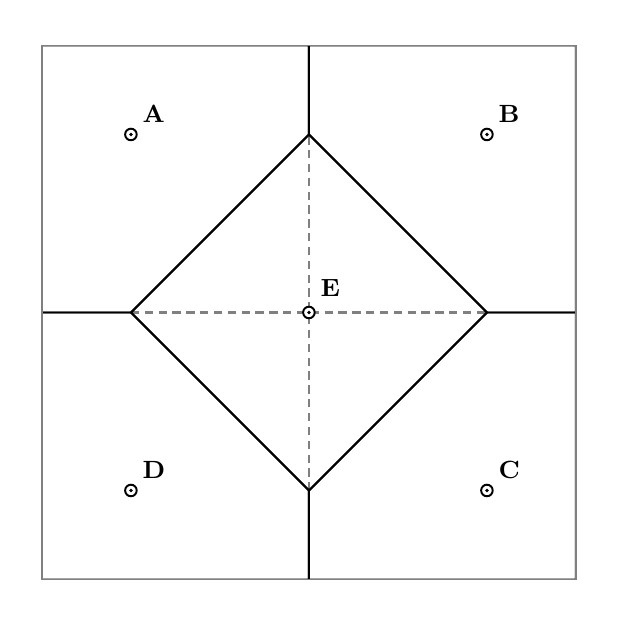
\begin{tikzpicture}[x=.445in,y=.445in]
\path[use as bounding box] (-3.16,-3.2) rectangle (3.2,3.2);
\begin{scope}
\clip (-3,-3) rectangle (3,3);
\draw[black!50,densely dashed,line width=.9pt] (-2,0)--(2,0) (0,-2)--(0,2);
\draw[line width=.7pt] (0.00000000,2.00000000)--(0.00000000,3.00000000)--(-3.00000000,3.00000000)--(-3.00000000,0.00000000)--(-2.00000000,0.00000000)--cycle;
\draw[line width=.7pt] (3.00000000,0.00000000)--(3.00000000,3.00000000)--(0.00000000,3.00000000)--(0.00000000,2.00000000)--(2.00000000,0.00000000)--cycle;
\draw[line width=.7pt] (0.00000000,-3.00000000)--(3.00000000,-3.00000000)--(3.00000000,0.00000000)--(2.00000000,0.00000000)--(0.00000000,-2.00000000)--cycle;
\draw[line width=.7pt] (-3.00000000,-3.00000000)--(0.00000000,-3.00000000)--(0.00000000,-2.00000000)--(-2.00000000,0.00000000)--(-3.00000000,0.00000000)--cycle;
\draw[line width=.7pt] (0.00000000,-2.00000000)--(2.00000000,0.00000000)--(0.00000000,2.00000000)--(-2.00000000,0.00000000)--cycle;

\end{scope}
\draw[black!50,line width=.5pt] (-3,-3) rectangle (3,3);
\draw[fill=white,line width=.7pt] (-2.00000000,2.00000000) circle[radius=.065];
\fill (-2.00000000,2.00000000) circle[radius=.021];
\node[anchor=south west,fill=white,inner sep=.8pt,font=\bfseries\fontsize{9}{10}\selectfont] at (-1.9,2.1) {A};
\draw[fill=white,line width=.7pt] (2.00000000,2.00000000) circle[radius=.065];
\fill (2.00000000,2.00000000) circle[radius=.021];
\node[anchor=south west,fill=white,inner sep=.8pt,font=\bfseries\fontsize{9}{10}\selectfont] at (2.1,2.1) {B};
\draw[fill=white,line width=.7pt] (2.00000000,-2.00000000) circle[radius=.065];
\fill (2.00000000,-2.00000000) circle[radius=.021];
\node[anchor=south west,fill=white,inner sep=.8pt,font=\bfseries\fontsize{9}{10}\selectfont] at (2.1,-1.9) {C};
\draw[fill=white,line width=.7pt] (-2.00000000,-2.00000000) circle[radius=.065];
\fill (-2.00000000,-2.00000000) circle[radius=.021];
\node[anchor=south west,fill=white,inner sep=.8pt,font=\bfseries\fontsize{9}{10}\selectfont] at (-1.9,-1.9) {D};
\draw[fill=white,line width=.7pt] (0.00000000,0.00000000) circle[radius=.065];
\fill (0.00000000,0.00000000) circle[radius=.021];
\node[anchor=south west,fill=white,inner sep=.8pt,font=\bfseries\fontsize{9}{10}\selectfont] at (0.1,0.15) {E};
\end{tikzpicture}
\par\raggedright\fontsize{9}{11}\selectfont Dashed cross: erased old boundaries. Solid diamond edges: new shared ties.
\end{minipage}
\vspace{.15in}
\newpage
{\Large\bfseries Grades 2--3 solutions}\par
\vspace{.08in}
{\large\bfseries Problem 7 Share with two regions and avoid the third}\par
\vspace{3pt}
\noindent\begin{minipage}[t]{.58\textwidth}\vspace{0pt}
\fontsize{10.8}{13.2}\selectfont
\textbf{Solution.} One successful choice is D at $(0,-5/2)$. It gets $y\leq-4|x|/5-9/20$. It shares the two lower sloping rays with A and B, and no point with C.

\textbf{Reasoning.} The new ABD vertex is $(0,-9/20)$, below the old ABC vertex $(0,0)$. The AB edge connects them. C still has $y\geq|x|$, leaving a gap between C and D. Putting D at $(0,-2)$ fails: D then shares the center with C.

\textbf{Hint to hold.} If D touches C at the center, move D a little farther down and rebuild the comparisons.

\textbf{Optional extension.} For a centered D at $(0,-t)$, the construction works whenever $2<t\leq3$.
\end{minipage}\hfill\begin{minipage}[t]{.40\textwidth}\vspace{0pt}\centering
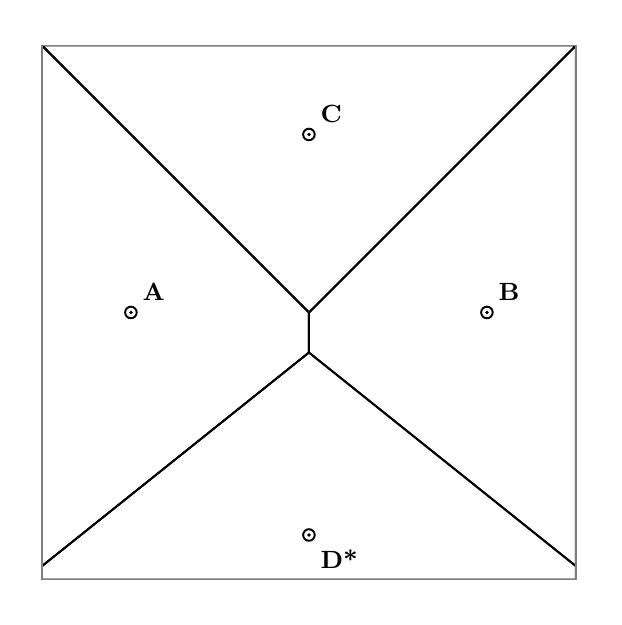
\begin{tikzpicture}[x=.445in,y=.445in]
\path[use as bounding box] (-3.16,-3.2) rectangle (3.2,3.2);
\begin{scope}
\clip (-3,-3) rectangle (3,3);
\draw[line width=.7pt] (0.00000000,-0.45000000)--(0.00000000,0.00000000)--(-3.00000000,3.00000000)--(-3.00000000,-2.85000000)--cycle;
\draw[line width=.7pt] (3.00000000,-2.85000000)--(3.00000000,3.00000000)--(0.00000000,0.00000000)--(0.00000000,-0.45000000)--cycle;
\draw[line width=.7pt] (3.00000000,3.00000000)--(-3.00000000,3.00000000)--(0.00000000,0.00000000)--cycle;
\draw[line width=.7pt] (-3.00000000,-3.00000000)--(3.00000000,-3.00000000)--(3.00000000,-2.85000000)--(0.00000000,-0.45000000)--(-3.00000000,-2.85000000)--cycle;

\end{scope}
\draw[black!50,line width=.5pt] (-3,-3) rectangle (3,3);
\draw[fill=white,line width=.7pt] (-2.00000000,0.00000000) circle[radius=.065];
\fill (-2.00000000,0.00000000) circle[radius=.021];
\node[anchor=south west,fill=white,inner sep=.8pt,font=\bfseries\fontsize{9}{10}\selectfont] at (-1.9,0.1) {A};
\draw[fill=white,line width=.7pt] (2.00000000,0.00000000) circle[radius=.065];
\fill (2.00000000,0.00000000) circle[radius=.021];
\node[anchor=south west,fill=white,inner sep=.8pt,font=\bfseries\fontsize{9}{10}\selectfont] at (2.1,0.1) {B};
\draw[fill=white,line width=.7pt] (0.00000000,2.00000000) circle[radius=.065];
\fill (0.00000000,2.00000000) circle[radius=.021];
\node[anchor=south west,fill=white,inner sep=.8pt,font=\bfseries\fontsize{9}{10}\selectfont] at (0.1,2.1) {C};
\draw[fill=white,line width=.7pt] (0.00000000,-2.50000000) circle[radius=.065];
\fill (0.00000000,-2.50000000) circle[radius=.021];
\node[anchor=north west,fill=white,inner sep=.8pt,font=\bfseries\fontsize{9}{10}\selectfont] at (0.1,-2.63) {D*};
\end{tikzpicture}
\par\raggedright\fontsize{9}{11}\selectfont A: $x\leq0,\ 4x/5-9/20\leq y\leq-x$; B is its mirror.
\end{minipage}
\vfill
{\large\bfseries Problem 8 Make a corner region}\par
\vspace{3pt}
\noindent\begin{minipage}[t]{.58\textwidth}\vspace{0pt}
\fontsize{10.8}{13.2}\selectfont
\textbf{Solution.} Put B at $(2,0)$ and C at $(0,2)$, or exchange their names. A gets $x\leq1$ and $y\leq1$, exactly the target inside the frame. B gets $x\geq1,y\leq x$; C gets $y\geq1,y\geq x$.

\textbf{Reasoning.} Reflect A across each of the two interior target edges. The remaining B/C boundary is the ray $y=x,x\geq1$. All three cells meet at $(1,1)$.

\textbf{Hint to hold.} Which printed edges really separate owners, and which are merely the frame?

\textbf{Optional extension.} Extend the paper mentally: explain why A does not have a bounded square cell.
\end{minipage}\hfill\begin{minipage}[t]{.40\textwidth}\vspace{0pt}\centering
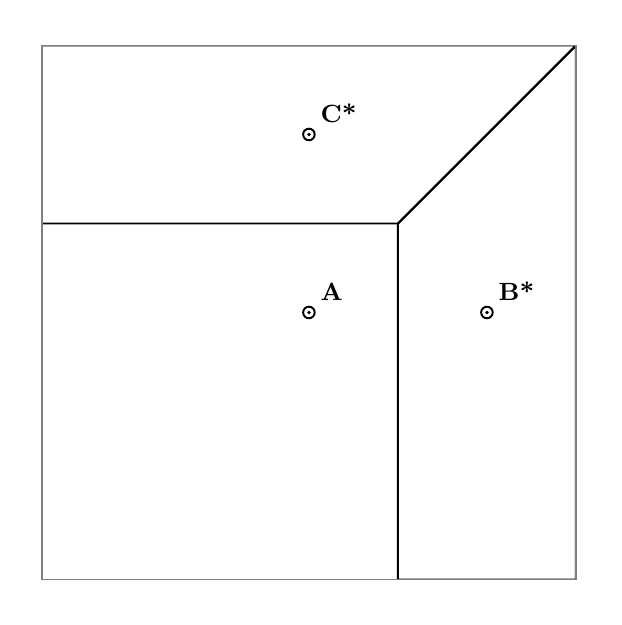
\begin{tikzpicture}[x=.445in,y=.445in]
\path[use as bounding box] (-3.16,-3.2) rectangle (3.2,3.2);
\begin{scope}
\clip (-3,-3) rectangle (3,3);
\draw[line width=.7pt] (-3.00000000,-3.00000000)--(1.00000000,-3.00000000)--(1.00000000,1.00000000)--(-3.00000000,1.00000000)--cycle;
\draw[line width=.7pt] (1.00000000,-3.00000000)--(3.00000000,-3.00000000)--(3.00000000,3.00000000)--(1.00000000,1.00000000)--cycle;
\draw[line width=.7pt] (3.00000000,3.00000000)--(-3.00000000,3.00000000)--(-3.00000000,1.00000000)--(1.00000000,1.00000000)--cycle;

\end{scope}
\draw[black!50,line width=.5pt] (-3,-3) rectangle (3,3);
\draw[fill=white,line width=.7pt] (0.00000000,0.00000000) circle[radius=.065];
\fill (0.00000000,0.00000000) circle[radius=.021];
\node[anchor=south west,fill=white,inner sep=.8pt,font=\bfseries\fontsize{9}{10}\selectfont] at (0.1,0.1) {A};
\draw[fill=white,line width=.7pt] (2.00000000,0.00000000) circle[radius=.065];
\fill (2.00000000,0.00000000) circle[radius=.021];
\node[anchor=south west,fill=white,inner sep=.8pt,font=\bfseries\fontsize{9}{10}\selectfont] at (2.1,0.1) {B*};
\draw[fill=white,line width=.7pt] (0.00000000,2.00000000) circle[radius=.065];
\fill (0.00000000,2.00000000) circle[radius=.021];
\node[anchor=south west,fill=white,inner sep=.8pt,font=\bfseries\fontsize{9}{10}\selectfont] at (0.1,2.1) {C*};
\end{tikzpicture}
\par\raggedright\fontsize{9}{11}\selectfont The left and bottom frame edges do not bound A\textquotesingle s whole region.
\end{minipage}
\vspace{.15in}
\newpage
{\Large\bfseries Grades 4--5 solutions}\par
\vspace{.08in}
{\large\bfseries Problem 1 Certify the whole two-site map}\par
\vspace{3pt}
\noindent\begin{minipage}[t]{.58\textwidth}\vspace{0pt}
\fontsize{10.8}{13.2}\selectfont
\textbf{Solution.} The boundary is $3x+2y=0$. A owns $3x+2y\leq0$; B owns $3x+2y\geq0$. Every crease point is shared.

\textbf{Reasoning.} Folding A onto B proves equality on the crease. On A\textquotesingle s side, the segment to B crosses the crease at T. Since $TA=TB$, the triangle inequality gives $XA\leq XT+TA=XB$, with strict inequality off the crease. The opposite side is symmetric.

\textbf{Hint to hold.} Use reflection to explain points not tested with a string.

\textbf{Optional extension.} Explain why measuring fifty points would still leave other points untested.
\end{minipage}\hfill\begin{minipage}[t]{.40\textwidth}\vspace{0pt}\centering
\begin{tikzpicture}[x=.445in,y=.445in]
\path[use as bounding box] (-3.16,-3.2) rectangle (3.2,3.2);
\begin{scope}
\clip (-3,-3) rectangle (3,3);
\draw[line width=.7pt] (-3.00000000,-3.00000000)--(2.00000000,-3.00000000)--(-2.00000000,3.00000000)--(-3.00000000,3.00000000)--cycle;
\draw[line width=.7pt] (2.00000000,-3.00000000)--(3.00000000,-3.00000000)--(3.00000000,3.00000000)--(-2.00000000,3.00000000)--cycle;

\end{scope}
\draw[black!50,line width=.5pt] (-3,-3) rectangle (3,3);
\draw[fill=white,line width=.7pt] (-1.50000000,-1.00000000) circle[radius=.065];
\fill (-1.50000000,-1.00000000) circle[radius=.021];
\node[anchor=south west,fill=white,inner sep=.8pt,font=\bfseries\fontsize{9}{10}\selectfont] at (-1.4,-0.9) {A};
\draw[fill=white,line width=.7pt] (1.50000000,1.00000000) circle[radius=.065];
\fill (1.50000000,1.00000000) circle[radius=.021];
\node[anchor=south west,fill=white,inner sep=.8pt,font=\bfseries\fontsize{9}{10}\selectfont] at (1.6,1.1) {B};
\end{tikzpicture}
\par\raggedright\fontsize{9}{11}\selectfont A perpendicular bisector certifies infinitely many comparisons at once.
\end{minipage}
\vfill
{\large\bfseries Problem 2 Keep only nearest ties}\par
\vspace{3pt}
\noindent\begin{minipage}[t]{.58\textwidth}\vspace{0pt}
\fontsize{10.8}{13.2}\selectfont
\textbf{Solution.} A gets $x\leq0,y\leq-x$; B gets $x\geq0,y\leq x$; C gets $y\geq|x|$. The three surviving rays meet at the origin.

\textbf{Reasoning.} A pairwise bisector is only a candidate boundary: retain the parts where no other site is closer than the tied pair. The positive $y$-axis fails this test because C is nearer; the three surviving rays include their three-way meeting point.

\textbf{Hint to hold.} On each proposed boundary, try a point on either side of the three-way meeting.

\textbf{Optional extension.} Draw a circle centered at the triple tie through all three sites. What would a site inside it do?
\end{minipage}\hfill\begin{minipage}[t]{.40\textwidth}\vspace{0pt}\centering
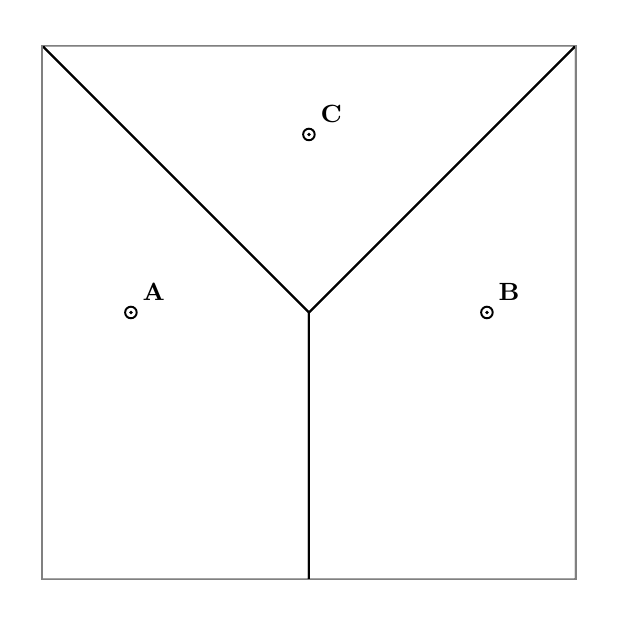
\begin{tikzpicture}[x=.445in,y=.445in]
\path[use as bounding box] (-3.16,-3.2) rectangle (3.2,3.2);
\begin{scope}
\clip (-3,-3) rectangle (3,3);
\draw[line width=.7pt] (-3.00000000,-3.00000000)--(0.00000000,-3.00000000)--(0.00000000,0.00000000)--(-3.00000000,3.00000000)--cycle;
\draw[line width=.7pt] (0.00000000,-3.00000000)--(3.00000000,-3.00000000)--(3.00000000,3.00000000)--(0.00000000,0.00000000)--cycle;
\draw[line width=.7pt] (3.00000000,3.00000000)--(-3.00000000,3.00000000)--(0.00000000,0.00000000)--cycle;

\end{scope}
\draw[black!50,line width=.5pt] (-3,-3) rectangle (3,3);
\draw[fill=white,line width=.7pt] (-2.00000000,0.00000000) circle[radius=.065];
\fill (-2.00000000,0.00000000) circle[radius=.021];
\node[anchor=south west,fill=white,inner sep=.8pt,font=\bfseries\fontsize{9}{10}\selectfont] at (-1.9,0.1) {A};
\draw[fill=white,line width=.7pt] (2.00000000,0.00000000) circle[radius=.065];
\fill (2.00000000,0.00000000) circle[radius=.021];
\node[anchor=south west,fill=white,inner sep=.8pt,font=\bfseries\fontsize{9}{10}\selectfont] at (2.1,0.1) {B};
\draw[fill=white,line width=.7pt] (0.00000000,2.00000000) circle[radius=.065];
\fill (0.00000000,2.00000000) circle[radius=.021];
\node[anchor=south west,fill=white,inner sep=.8pt,font=\bfseries\fontsize{9}{10}\selectfont] at (0.1,2.1) {C};
\end{tikzpicture}
\par\raggedright\fontsize{9}{11}\selectfont The positive $y$-axis is an A/B equality, but is not a nearest-site boundary.
\end{minipage}
\vspace{.15in}
\newpage
{\Large\bfseries Grades 4--5 solutions}\par
\vspace{.08in}
{\large\bfseries Problem 3 A whole bounded cell}\par
\vspace{3pt}
\noindent\begin{minipage}[t]{.58\textwidth}\vspace{0pt}
\fontsize{10.8}{13.2}\selectfont
\textbf{Solution.} D gets the triangle with vertices $(-7/4,1)$, $(7/4,1)$ and $(0,-5/2)$. Its inequalities are $y\leq1$ and $y\geq2|x|-5/2$. No joining segment can leave it.

\textbf{Reasoning.} D must stay on its winning side against each of A, B and C. Each allowed half-plane contains the entire segment between any two of its points. A segment between two points allowed by all three comparisons therefore stays allowed by all three.

\textbf{Hint to hold.} Trace each allowed side on a separate sheet, then overlap the sheets.

\textbf{Optional extension.} The same argument works for any finite set of distinct point sites. Invite a child to explain that generalization.
\end{minipage}\hfill\begin{minipage}[t]{.40\textwidth}\vspace{0pt}\centering
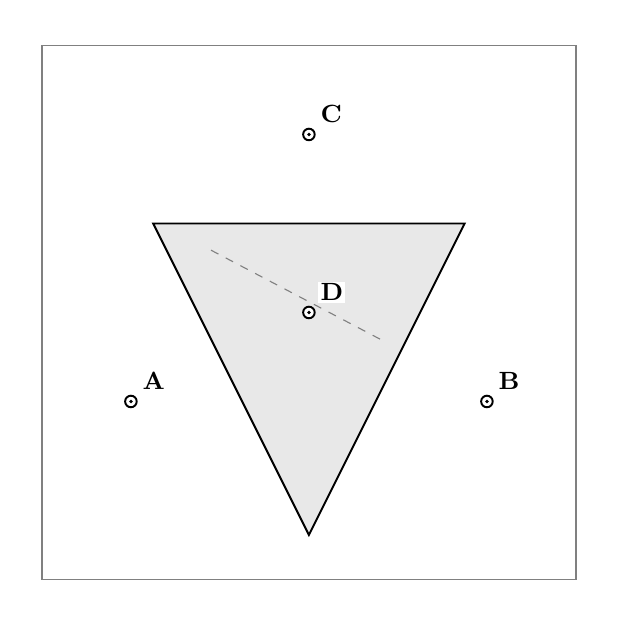
\begin{tikzpicture}[x=.445in,y=.445in]
\path[use as bounding box] (-3.16,-3.2) rectangle (3.2,3.2);
\fill[black!9] (-1.75000000,1.00000000)--(0.00000000,-2.50000000)--(1.75000000,1.00000000)--cycle;
\begin{scope}
\clip (-3,-3) rectangle (3,3);
\draw[line width=.7pt] (-1.75000000,1.00000000)--(0.00000000,-2.50000000)--(1.75000000,1.00000000)--cycle;
\draw[black!50,dashed] (-1.10000000,0.70000000)--(0.80000000,-0.30000000);

\end{scope}
\draw[black!50,line width=.5pt] (-3,-3) rectangle (3,3);
\draw[fill=white,line width=.7pt] (-2.00000000,-1.00000000) circle[radius=.065];
\fill (-2.00000000,-1.00000000) circle[radius=.021];
\node[anchor=south west,fill=white,inner sep=.8pt,font=\bfseries\fontsize{9}{10}\selectfont] at (-1.9,-0.9) {A};
\draw[fill=white,line width=.7pt] (2.00000000,-1.00000000) circle[radius=.065];
\fill (2.00000000,-1.00000000) circle[radius=.021];
\node[anchor=south west,fill=white,inner sep=.8pt,font=\bfseries\fontsize{9}{10}\selectfont] at (2.1,-0.9) {B};
\draw[fill=white,line width=.7pt] (0.00000000,2.00000000) circle[radius=.065];
\fill (0.00000000,2.00000000) circle[radius=.021];
\node[anchor=south west,fill=white,inner sep=.8pt,font=\bfseries\fontsize{9}{10}\selectfont] at (0.1,2.1) {C};
\draw[fill=white,line width=.7pt] (0.00000000,0.00000000) circle[radius=.065];
\fill (0.00000000,0.00000000) circle[radius=.021];
\node[anchor=south west,fill=white,inner sep=.8pt,font=\bfseries\fontsize{9}{10}\selectfont] at (0.1,0.1) {D};
\end{tikzpicture}
\par\raggedright\fontsize{9}{11}\selectfont The shaded triangle is D\textquotesingle s entire cell, not merely its part inside the frame.
\end{minipage}
\vfill
{\large\bfseries Problem 4 A four-way meeting}\par
\vspace{3pt}
\noindent\begin{minipage}[t]{.58\textwidth}\vspace{0pt}
\fontsize{10.8}{13.2}\selectfont
\textbf{Solution.} The cells are the four closed quarters. The origin is the only place shared by three or more sites; it is shared by all four. Elsewhere on an axis there are exactly two nearest sites.

\textbf{Reasoning.} The four sites lie on one circle centered at the origin. An AB equality requires $x=0$, and a tie with D also requires $y=0$, fixing the point. The same point also ties C.

\textbf{Hint to hold.} Look for the center of a circle through the sites.

\textbf{Optional extension.} Explain why saying ``three regions always meet at a vertex\textquotesingle\textquotesingle\ is false. Compare the perturbed square in grades 2--3 Problem 5.
\end{minipage}\hfill\begin{minipage}[t]{.40\textwidth}\vspace{0pt}\centering
\begin{tikzpicture}[x=.445in,y=.445in]
\path[use as bounding box] (-3.16,-3.2) rectangle (3.2,3.2);
\begin{scope}
\clip (-3,-3) rectangle (3,3);
\draw[line width=.7pt] (0.00000000,0.00000000)--(0.00000000,3.00000000)--(-3.00000000,3.00000000)--(-3.00000000,0.00000000)--cycle;
\draw[line width=.7pt] (3.00000000,0.00000000)--(3.00000000,3.00000000)--(0.00000000,3.00000000)--(0.00000000,0.00000000)--cycle;
\draw[line width=.7pt] (0.00000000,-3.00000000)--(3.00000000,-3.00000000)--(3.00000000,0.00000000)--(0.00000000,0.00000000)--cycle;
\draw[line width=.7pt] (-3.00000000,-3.00000000)--(0.00000000,-3.00000000)--(0.00000000,0.00000000)--(-3.00000000,0.00000000)--cycle;

\end{scope}
\draw[black!50,line width=.5pt] (-3,-3) rectangle (3,3);
\draw[fill=white,line width=.7pt] (-2.00000000,2.00000000) circle[radius=.065];
\fill (-2.00000000,2.00000000) circle[radius=.021];
\node[anchor=south west,fill=white,inner sep=.8pt,font=\bfseries\fontsize{9}{10}\selectfont] at (-1.9,2.1) {A};
\draw[fill=white,line width=.7pt] (2.00000000,2.00000000) circle[radius=.065];
\fill (2.00000000,2.00000000) circle[radius=.021];
\node[anchor=south west,fill=white,inner sep=.8pt,font=\bfseries\fontsize{9}{10}\selectfont] at (2.1,2.1) {B};
\draw[fill=white,line width=.7pt] (2.00000000,-2.00000000) circle[radius=.065];
\fill (2.00000000,-2.00000000) circle[radius=.021];
\node[anchor=south west,fill=white,inner sep=.8pt,font=\bfseries\fontsize{9}{10}\selectfont] at (2.1,-1.9) {C};
\draw[fill=white,line width=.7pt] (-2.00000000,-2.00000000) circle[radius=.065];
\fill (-2.00000000,-2.00000000) circle[radius=.021];
\node[anchor=south west,fill=white,inner sep=.8pt,font=\bfseries\fontsize{9}{10}\selectfont] at (-1.9,-1.9) {D};
\end{tikzpicture}
\par\raggedright\fontsize{9}{11}\selectfont A four-way tie is intentional; no general-position assumption is in force.
\end{minipage}
\vspace{.15in}
\newpage
{\Large\bfseries Grades 4--5 solutions}\par
\vspace{.08in}
{\large\bfseries Problem 5 Insertion can only shrink}\par
\vspace{3pt}
\noindent\begin{minipage}[t]{.58\textwidth}\vspace{0pt}
\fontsize{10.8}{13.2}\selectfont
\textbf{Solution.} E gets the diamond $|x|+|y|\leq2$. Each old region is its old quarter cut by $|x|+|y|\geq2$. Erase the old axis pieces with distance from the origin strictly less than 2; keep the four endpoint ties.

\textbf{Reasoning.} For an old site A, its new region is its old region intersected with the additional condition $d(X,A)\leq d(X,E)$. An intersection cannot add points. Some regions may stay unchanged; none can grow.

\textbf{Hint to hold.} Ask whether an old loser can become a winner merely because one more competitor appears.

\textbf{Optional extension.} Could removing a site shrink an old region? Reverse the comparison argument.
\end{minipage}\hfill\begin{minipage}[t]{.40\textwidth}\vspace{0pt}\centering
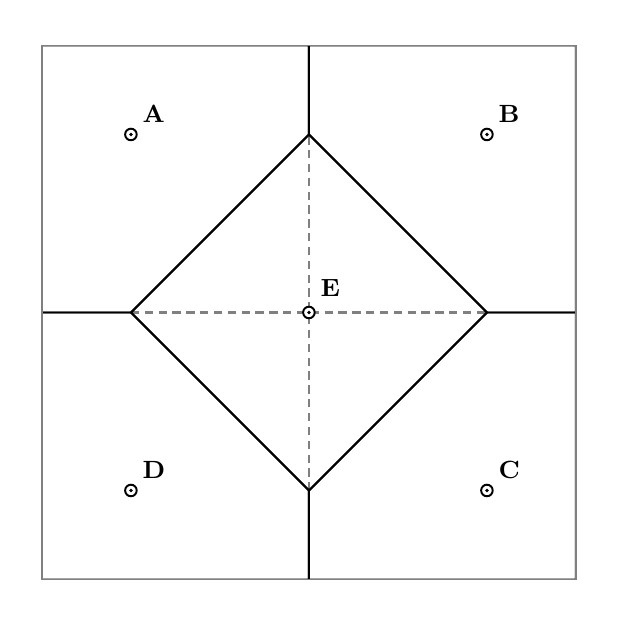
\begin{tikzpicture}[x=.445in,y=.445in]
\path[use as bounding box] (-3.16,-3.2) rectangle (3.2,3.2);
\begin{scope}
\clip (-3,-3) rectangle (3,3);
\draw[black!50,densely dashed,line width=.9pt] (-2,0)--(2,0) (0,-2)--(0,2);
\draw[line width=.7pt] (0.00000000,2.00000000)--(0.00000000,3.00000000)--(-3.00000000,3.00000000)--(-3.00000000,0.00000000)--(-2.00000000,0.00000000)--cycle;
\draw[line width=.7pt] (3.00000000,0.00000000)--(3.00000000,3.00000000)--(0.00000000,3.00000000)--(0.00000000,2.00000000)--(2.00000000,0.00000000)--cycle;
\draw[line width=.7pt] (0.00000000,-3.00000000)--(3.00000000,-3.00000000)--(3.00000000,0.00000000)--(2.00000000,0.00000000)--(0.00000000,-2.00000000)--cycle;
\draw[line width=.7pt] (-3.00000000,-3.00000000)--(0.00000000,-3.00000000)--(0.00000000,-2.00000000)--(-2.00000000,0.00000000)--(-3.00000000,0.00000000)--cycle;
\draw[line width=.7pt] (0.00000000,-2.00000000)--(2.00000000,0.00000000)--(0.00000000,2.00000000)--(-2.00000000,0.00000000)--cycle;

\end{scope}
\draw[black!50,line width=.5pt] (-3,-3) rectangle (3,3);
\draw[fill=white,line width=.7pt] (-2.00000000,2.00000000) circle[radius=.065];
\fill (-2.00000000,2.00000000) circle[radius=.021];
\node[anchor=south west,fill=white,inner sep=.8pt,font=\bfseries\fontsize{9}{10}\selectfont] at (-1.9,2.1) {A};
\draw[fill=white,line width=.7pt] (2.00000000,2.00000000) circle[radius=.065];
\fill (2.00000000,2.00000000) circle[radius=.021];
\node[anchor=south west,fill=white,inner sep=.8pt,font=\bfseries\fontsize{9}{10}\selectfont] at (2.1,2.1) {B};
\draw[fill=white,line width=.7pt] (2.00000000,-2.00000000) circle[radius=.065];
\fill (2.00000000,-2.00000000) circle[radius=.021];
\node[anchor=south west,fill=white,inner sep=.8pt,font=\bfseries\fontsize{9}{10}\selectfont] at (2.1,-1.9) {C};
\draw[fill=white,line width=.7pt] (-2.00000000,-2.00000000) circle[radius=.065];
\fill (-2.00000000,-2.00000000) circle[radius=.021];
\node[anchor=south west,fill=white,inner sep=.8pt,font=\bfseries\fontsize{9}{10}\selectfont] at (-1.9,-1.9) {D};
\draw[fill=white,line width=.7pt] (0.00000000,0.00000000) circle[radius=.065];
\fill (0.00000000,0.00000000) circle[radius=.021];
\node[anchor=south west,fill=white,inner sep=.8pt,font=\bfseries\fontsize{9}{10}\selectfont] at (0.1,0.15) {E};
\end{tikzpicture}
\par\raggedright\fontsize{9}{11}\selectfont The diamond vertices are ABE, BCE, CDE and ADE, in clockwise order from the top.
\end{minipage}
\vfill
{\large\bfseries Problem 6 The fewest sites to close a strip}\par
\vspace{3pt}
\noindent\begin{minipage}[t]{.58\textwidth}\vspace{0pt}
\fontsize{10.8}{13.2}\selectfont
\textbf{Solution.} Two new dots suffice: D at $(0,2)$ and E at $(0,-2)$. B then gets exactly $[-1,1]\times[-1,1]$, entirely inside the frame. One new dot cannot work.

\textbf{Reasoning.} Originally B owns the unbounded vertical strip $|x|\leq1$. One new site contributes only one half-plane. If its height is positive, a downward vertical tail remains; if negative, an upward tail remains; if zero, a full vertical line remains. Thus at least two are necessary.

\textbf{Hint to hold.} After trying one new dot, follow B\textquotesingle s region beyond the top and bottom of the picture.

\textbf{Optional extension.} Find another pair that makes B a bounded quadrilateral.
\end{minipage}\hfill\begin{minipage}[t]{.40\textwidth}\vspace{0pt}\centering
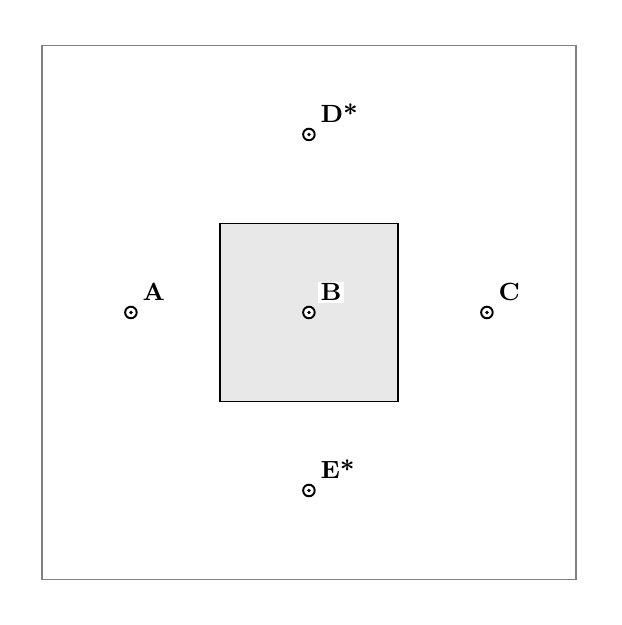
\begin{tikzpicture}[x=.445in,y=.445in]
\path[use as bounding box] (-3.16,-3.2) rectangle (3.2,3.2);
\fill[black!9] (1.00000000,-1.00000000)--(1.00000000,1.00000000)--(-1.00000000,1.00000000)--(-1.00000000,-1.00000000)--cycle;
\begin{scope}
\clip (-3,-3) rectangle (3,3);
\draw[line width=.7pt] (1.00000000,-1.00000000)--(1.00000000,1.00000000)--(-1.00000000,1.00000000)--(-1.00000000,-1.00000000)--cycle;

\end{scope}
\draw[black!50,line width=.5pt] (-3,-3) rectangle (3,3);
\draw[fill=white,line width=.7pt] (-2.00000000,0.00000000) circle[radius=.065];
\fill (-2.00000000,0.00000000) circle[radius=.021];
\node[anchor=south west,fill=white,inner sep=.8pt,font=\bfseries\fontsize{9}{10}\selectfont] at (-1.9,0.1) {A};
\draw[fill=white,line width=.7pt] (0.00000000,0.00000000) circle[radius=.065];
\fill (0.00000000,0.00000000) circle[radius=.021];
\node[anchor=south west,fill=white,inner sep=.8pt,font=\bfseries\fontsize{9}{10}\selectfont] at (0.1,0.1) {B};
\draw[fill=white,line width=.7pt] (2.00000000,0.00000000) circle[radius=.065];
\fill (2.00000000,0.00000000) circle[radius=.021];
\node[anchor=south west,fill=white,inner sep=.8pt,font=\bfseries\fontsize{9}{10}\selectfont] at (2.1,0.1) {C};
\draw[fill=white,line width=.7pt] (0.00000000,2.00000000) circle[radius=.065];
\fill (0.00000000,2.00000000) circle[radius=.021];
\node[anchor=south west,fill=white,inner sep=.8pt,font=\bfseries\fontsize{9}{10}\selectfont] at (0.1,2.1) {D*};
\draw[fill=white,line width=.7pt] (0.00000000,-2.00000000) circle[radius=.065];
\fill (0.00000000,-2.00000000) circle[radius=.021];
\node[anchor=south west,fill=white,inner sep=.8pt,font=\bfseries\fontsize{9}{10}\selectfont] at (0.1,-1.9) {E*};
\end{tikzpicture}
\par\raggedright\fontsize{9}{11}\selectfont D* and E* are added. The frame is $[-3,3]^2$; it does not itself stop a region.
\end{minipage}
\vspace{.15in}
\newpage
{\Large\bfseries Grades 4--5 solutions}\par
\vspace{.08in}
{\large\bfseries Problem 7 Build the prescribed triangle}\par
\vspace{3pt}
\noindent\begin{minipage}[t]{.58\textwidth}\vspace{0pt}
\fontsize{10.8}{13.2}\selectfont
\textbf{Solution.} Reflect A across each target side. One labeling is B$=(0,-2)$, C$=(24/13,16/13)$ and D$=(-24/13,16/13)$. All three new dots fit in the frame.

\textbf{Reasoning.} The three winning comparisons are $y\geq-1$, $3x+2y\leq4$, and $-3x+2y\leq4$. Their intersection has exactly the target vertices $(-2,-1)$, $(2,-1)$ and $(0,2)$. No additional constraint appears.

\textbf{Hint to hold.} Fold on one target edge and mark where A lands; repeat independently for the other two.

\textbf{Optional extension.} Can the same reflection construction make a different convex polygon around A?
\end{minipage}\hfill\begin{minipage}[t]{.40\textwidth}\vspace{0pt}\centering
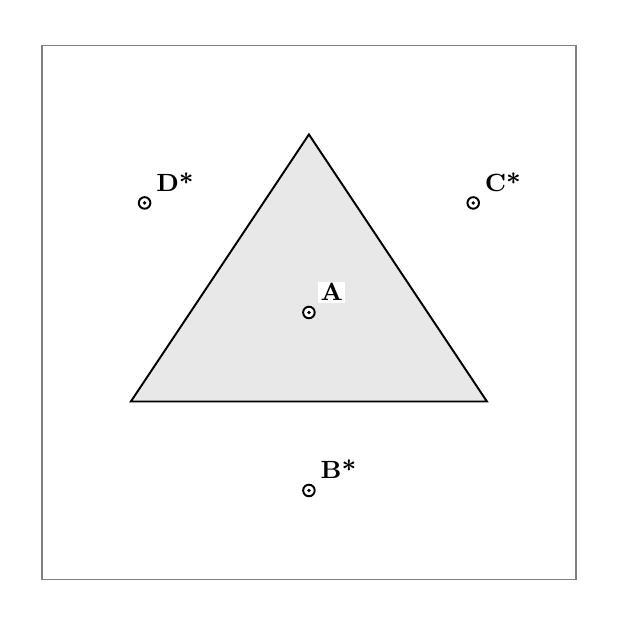
\begin{tikzpicture}[x=.445in,y=.445in]
\path[use as bounding box] (-3.16,-3.2) rectangle (3.2,3.2);
\fill[black!9] (-2.00000000,-1.00000000)--(2.00000000,-1.00000000)--(0.00000000,2.00000000)--cycle;
\begin{scope}
\clip (-3,-3) rectangle (3,3);
\draw[line width=.7pt] (-2.00000000,-1.00000000)--(2.00000000,-1.00000000)--(0.00000000,2.00000000)--cycle;

\end{scope}
\draw[black!50,line width=.5pt] (-3,-3) rectangle (3,3);
\draw[fill=white,line width=.7pt] (0.00000000,0.00000000) circle[radius=.065];
\fill (0.00000000,0.00000000) circle[radius=.021];
\node[anchor=south west,fill=white,inner sep=.8pt,font=\bfseries\fontsize{9}{10}\selectfont] at (0.1,0.1) {A};
\draw[fill=white,line width=.7pt] (0.00000000,-2.00000000) circle[radius=.065];
\fill (0.00000000,-2.00000000) circle[radius=.021];
\node[anchor=south west,fill=white,inner sep=.8pt,font=\bfseries\fontsize{9}{10}\selectfont] at (0.1,-1.9) {B*};
\draw[fill=white,line width=.7pt] (1.84615385,1.23076923) circle[radius=.065];
\fill (1.84615385,1.23076923) circle[radius=.021];
\node[anchor=south west,fill=white,inner sep=.8pt,font=\bfseries\fontsize{9}{10}\selectfont] at (1.9461538461538463,1.330769230769231) {C*};
\draw[fill=white,line width=.7pt] (-1.84615385,1.23076923) circle[radius=.065];
\fill (-1.84615385,1.23076923) circle[radius=.021];
\node[anchor=south west,fill=white,inner sep=.8pt,font=\bfseries\fontsize{9}{10}\selectfont] at (-1.7461538461538462,1.330769230769231) {D*};
\end{tikzpicture}
\par\raggedright\fontsize{9}{11}\selectfont Each side is shared with its reflected site. The whole closed triangle belongs to A.
\end{minipage}
\vfill
{\large\bfseries Problem 8 A point that cannot be taken}\par
\vspace{3pt}
\noindent\begin{minipage}[t]{.58\textwidth}\vspace{0pt}
\fontsize{10.8}{13.2}\selectfont
\textbf{Solution.} R cannot be taken while P and Q still belong to A: R lies on segment PQ, and A\textquotesingle s cell is convex. S can be taken. Add B at $(0,-5/2)$; its bisector with A is $y=-1/4$.

\textbf{Reasoning.} A keeps $y\geq-1/4$, so P, Q and R remain strictly in A\textquotesingle s cell; S is strictly in B\textquotesingle s. At P and Q, squared distances are $8<41/4$; at S, $1/4<16$. Merely tying A at R would not remove R from A.

\textbf{Hint to hold.} For R, draw the segment PQ. For S, try a new dot below it.

\textbf{Optional extension.} Every point in triangle APQ must also remain with A. Why must A itself always remain?
\end{minipage}\hfill\begin{minipage}[t]{.40\textwidth}\vspace{0pt}\centering
\begin{tikzpicture}[x=.445in,y=.445in]
\path[use as bounding box] (-3.16,-3.2) rectangle (3.2,3.2);
\begin{scope}
\clip (-3,-3) rectangle (3,3);
\draw[line width=.7pt] (3.00000000,-0.25000000)--(3.00000000,3.00000000)--(-3.00000000,3.00000000)--(-3.00000000,-0.25000000)--cycle;
\draw[line width=.7pt] (-3.00000000,-3.00000000)--(3.00000000,-3.00000000)--(3.00000000,-0.25000000)--(-3.00000000,-0.25000000)--cycle;
\draw[black!50,dashed] (-2.00000000,0.00000000)--(2.00000000,0.00000000);

\end{scope}
\draw[black!50,line width=.5pt] (-3,-3) rectangle (3,3);
\draw[line width=.6pt] (-2.055,0)--(-1.945,0) (-2,-0.055)--(-2,0.055);
\node[anchor=south west,fill=white,inner sep=.8pt,font=\sffamily\fontsize{7.6}{8.4}\selectfont] at (-1.9,0.09) {P};
\draw[line width=.6pt] (1.945,0)--(2.055,0) (2,-0.055)--(2,0.055);
\node[anchor=south east,fill=white,inner sep=.8pt,font=\sffamily\fontsize{7.6}{8.4}\selectfont] at (1.9,0.09) {Q};
\draw[line width=.6pt] (-0.055,0)--(0.055,0) (0,-0.055)--(0,0.055);
\node[anchor=south west,fill=white,inner sep=.8pt,font=\sffamily\fontsize{7.6}{8.4}\selectfont] at (0.1,0.09) {R};
\draw[line width=.6pt] (-0.055,-2)--(0.055,-2) (0,-2.055)--(0,-1.945);
\node[anchor=south west,fill=white,inner sep=.8pt,font=\sffamily\fontsize{7.6}{8.4}\selectfont] at (0.1,-1.91) {S};
\draw[fill=white,line width=.7pt] (0.00000000,2.00000000) circle[radius=.065];
\fill (0.00000000,2.00000000) circle[radius=.021];
\node[anchor=south west,fill=white,inner sep=.8pt,font=\bfseries\fontsize{9}{10}\selectfont] at (0.1,2.1) {A};
\draw[fill=white,line width=.7pt] (0.00000000,-2.50000000) circle[radius=.065];
\fill (0.00000000,-2.50000000) circle[radius=.021];
\node[anchor=south west,fill=white,inner sep=.8pt,font=\bfseries\fontsize{9}{10}\selectfont] at (0.1,-2.4) {B*};
\end{tikzpicture}
\par\raggedright\fontsize{9}{11}\selectfont One successful construction for S; no construction works for R.
\end{minipage}
\vspace{.15in}
\end{document}